\documentclass{book}
\usepackage{amsfonts}
\usepackage{amsmath} % For math symbols
\usepackage{graphicx} % For including graphics
\usepackage{tikz}
\usepackage{tikz-3dplot} % For 3D graphics
\usepackage{pgfplots}
\usepackage{fancyhdr}
\usepackage{lipsum} % For dummy text
\usepackage{amsthm} % For theorem styles
\usepackage{enumitem}
\usepackage{xcolor}
\usepackage{multicol}
\usepackage{siunitx}
\usepackage{pgf-pie}
\usepackage{caption}
\usepackage{hyperref}
\hypersetup{
    colorlinks,
    citecolor=black,
    filecolor=black,
    linkcolor=blue,
    urlcolor=blue
}


\pgfplotsset{compat=1.17}
% Set up the fancyhdr package
\pagestyle{fancy}
\fancyhf{} % Clear all header and footer fields

% Define the header
% \fancyhead[LE,RO]{\thepage} % Page number on the left for even pages, right for odd pages
\fancyhead[RE]{\nouppercase{\leftmark}} % Chapter name on the right for even pages
\fancyhead[LO]{\nouppercase{\rightmark}} % Section name on the left for odd pages

% Define the footer (optional)
\fancyfoot[C]{\thepage} % Page number in the center of the footer

% Ensure chapter and section titles are in uppercase
\renewcommand{\chaptermark}[1]{\markboth{\thechapter.\ #1}{}}
\renewcommand{\sectionmark}[1]{\markright{\thesection.\ #1}}

\newtheoremstyle{examplestyle}
  {}{}{\itshape}{}{\bfseries}{.}{ }{\thmname{#1}\thmnumber{ #2}: \thmnote{ #3}}
\theoremstyle{examplestyle}
\newtheorem{example}{Example}

\begin{document}


\title{Mastering Mathematics: From Foundations to Infinite Possibilities}
\author{[Denzil James Greenwood]}
\date{\today}
\maketitle

\tableofcontents

\chapter{Introduction: The Beauty of Math for Everyone}
\section{Purpose of the Book}
Everyone can learn math. The purpose of this book is to simplify higher math and make it accessible to all learners, regardless of background or prior experience.
We will build from the foundations of basic math to the most advanced concepts, using clear explanations, real-life examples, and intuitive exercises.

\section{Overcoming Fear of Math}
Many people fear math because they think it's too hard or that they're just not good at it. This book takes a growth mindset approach, showing you that anyone can understand math by breaking down each concept step by step.

\section{The Language of Math}
We use math every day without even realizing it. This section will highlight how math is woven into our daily lives and why it's an essential language for understanding the world around us.
\chapter{Why Start Here? Addition and Subtraction}

Addition and subtraction are the building blocks of all mathematical concepts. If we think of math as a language, then addition and subtraction are the alphabet—simple yet powerful tools that help us solve problems, from everyday tasks to complex equations.

Let’s begin by understanding these basic operations deeply. Whether you’re managing your budget, dividing something between friends, or calculating distances, these two operations are always at play.


\section{What Is Addition?}
Addition is the process of combining two or more numbers to get a larger number. Think of it like this:
\begin{itemize}
    \item If you have 3 apples and someone gives you 2 more apples, how many apples do you have in total?
\end{itemize}
This problem is an example of addition: 3 apples + 2 apples = 5 apples.

Let’s look at some other simple examples:
\begin{itemize}
    \item 1 + 1 = 2
    \item 4 + 3 = 7
    \item 10 + 20 = 30
\end{itemize}

Addition works by combining. You start with one number, and as you add more numbers, the total grows.

\subsection{Visualizing Addition}
One of the best ways to understand addition is by using a number line. A number line is a straight line where numbers increase as you move to the right. To add, you simply move to the right by the number you're adding.

For example, if you’re adding 2 + 3, you can start at 2 on the number line and move 3 steps to the right. You’ll land at 5.

\begin{center}
    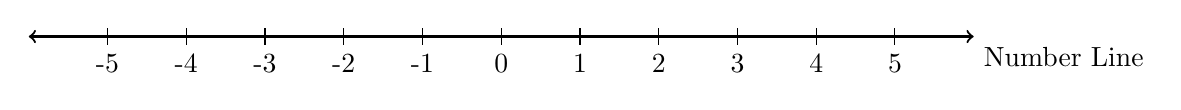
\begin{tikzpicture}
        \draw[thick, <->] (-6,0) -- (6,0) node[anchor=north west] {Number Line};
        \foreach \x in {-5,-4,-3,-2,-1,0,1,2,3,4,5}
            \draw (\x,3pt) -- (\x,-3pt) node[anchor=north] {\x};
    \end{tikzpicture}
    \end{center}

\section{What Is Subtraction?}
Subtraction is the process of taking one number away from another. If addition is about combining, subtraction is about removing.

For example:
\begin{itemize}
    \item You have 5 apples, and you give 2 away. How many apples are left?
\end{itemize}
This is subtraction: 5 apples - 2 apples = 3 apples.

Other simple examples:
\begin{itemize}
    \item 7 - 4 = 3
    \item 10 - 5 = 5
    \item 15 - 9 = 6
\end{itemize}

Subtraction helps us find out how much is left or how much we need to remove from something.

\subsection{Visualizing Subtraction}
We can also use a number line for subtraction. Instead of moving to the right as we do with addition, we move to the left.

If you’re subtracting 5 - 2, you start at 5 on the number line and move 2 steps to the left. You’ll land at 3.

\section{Practice Makes Perfect: Let’s Try Some Exercises!}
\subsection{Simple Addition}
\begin{enumerate}
    \item 5 + 4 = \_\_\_\_
    \item 7 + 2 = \_\_\_\_
    \item 10 + 6 = \_\_\_\_
    \item 3145 + 1234 = \_\_\_\_
    \item 100 + 1000 = \_\_\_\_
\end{enumerate}

\subsection{Simple Subtraction}
\begin{enumerate}
    \item 8 - 3 = \_\_\_\_
    \item 12 - 5 = \_\_\_\_
    \item 20 - 9 = \_\_\_\_
    \item 32 - 15 = \_\_\_\_
    \item 100 - 50 = \_\_\_\_
    \item 9534 - 1234 = \_\_\_\_
\end{enumerate}

Try to use a number line for these problems. Draw one out, and for each addition problem, move right. For each subtraction problem, move left. This will help you visualize the process.
\begin{center}
    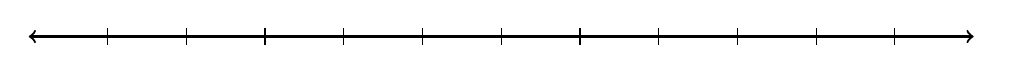
\begin{tikzpicture}
        \draw[thick, <->] (-6,0) -- (6,0) node[anchor=north west] {};
        \foreach \x in {-5,-4,-3,-2,-1,0,1,2,3,4,5}
            \draw (\x,3pt) -- (\x,-3pt);
    \end{tikzpicture}
\end{center}

\section{Making It Real: Addition and Subtraction in Everyday Life}
Math is everywhere. You use addition and subtraction more often than you think:
\begin{itemize}
    \item \textbf{Shopping:} You bought 3 oranges and added 2 apples to your basket. How many pieces of fruit do you have? That’s 3 + 2 = 5
    \item \textbf{Cooking:} You have 4 cups of flour, but your recipe only calls for 2 cups. How much flour will you have left after using what you need? That’s 4 - 2 = 2 cups left.
    \item \textbf{Traveling:} Your on a 20 mile trip you have traveled 15 miles. How many miles are left to go? That’s 20 - 15 = 5 miles left.
\end{itemize}

Addition and subtraction help you organize, plan, and make decisions in your daily life.

\section{The Properties of Addition and Subtraction}
Now that we’ve mastered the basics, let’s look at some important properties that will help us understand these operations even better:

\subsection{Commutative Property of Addition}
\begin{itemize}
    \item When adding two numbers, the order doesn’t matter.
    \item For example, 3 + 5 is the same as 5 + 3. Both equal 8.
\end{itemize}

\subsection{Associative Property of Addition}
\begin{itemize}
    \item When adding three or more numbers, it doesn’t matter how you group them.
    \item For example, (2 + 3) + 4 = 2 + (3 + 4). Both equal 9.
\end{itemize}

\subsection{Subtraction is not Commutative}
\begin{itemize}
    \item Unlike addition, the order does matter in subtraction.
    \item For example, 5 - 3 is not the same as 3 - 5. One equals 2, and the other equals -2.
\end{itemize}

\section{Breaking It Down: How to Approach Word Problems}
One of the most important ways math shows up in real life is through word problems. Word problems take a real-world situation and ask you to solve it with math.

Here’s a simple strategy to help you:
\begin{enumerate}
    \item Read the problem carefully.
    \item Identify what you’re being asked to find.
    \item Translate the words into numbers (e.g., “two more” means +2).
    \item Write down the math problem.
    \item Solve it!
\end{enumerate}

Let’s try an example:
\begin{itemize}
    \item \textbf{Problem:} Sarah has 5 marbles. She finds 3 more marbles. How many marbles does Sarah have now?
    \item \textbf{Step 1:} Identify what we know.
    \begin{enumerate}
        \item Sarah starts with 5 marbles.
        \item She finds 3 more.
    \end{enumerate}
    \item \textbf{Step 2:} Write the math problem:
    \begin{enumerate}
        \item 5 + 3 = 8.
    \end{enumerate}
    \item \textbf{Step 3:} Solve it. Sarah now has 8 marbles.
\end{itemize}

\section{Chapter Summary}
\begin{itemize}
    \item Addition is about combining numbers to get a larger total.
    \item Subtraction is about removing numbers to see how much is left.
    \item We can use number lines to help visualize both operations.
    \item These operations are useful in everyday life, from shopping to cooking and traveling.
    \item We learned the commutative and associative properties for addition and why subtraction doesn’t have these properties.
\end{itemize}
\section{Challenge Question}
Mastering addition and subtraction will set the stage for learning more advanced math concepts in the next chapters. Keep practicing, and soon you’ll be ready for the next step: multiplication and division!
\begin{enumerate}   
    \item You have 10 apples. You give 4 apples to your friend, and then you buy 5 more apples. How many apples do you have now?
    \begin{itemize}
        \item (10 - 4) + 5 = \_\_\_\_?
    \end{itemize}
    \item You have 15 candies. You eat 3 candies and then receive 7 more candies from a friend. How many candies do you have now?
    \begin{itemize}
        \item (15 - 3) + 7 = \_\_\_\_?
    \end{itemize}    
    \item You have 20 books. You lend 5 books to a friend and then buy 3 more books. How many books do you have now?
    \begin{itemize}
        \item (20 - 5) + 3 = \_\_\_\_?
    \end{itemize}
    \item You have 30 pencils. You give 10 pencils to your classmates and then find 8 more pencils. How many pencils do you have now?
    \begin{itemize}
        \item (30 - 10) + 8 = \_\_\_\_?
    \end{itemize}
    \item You have 50 stickers. You use 20 stickers and then receive 15 more stickers as a gift. How many stickers do you have now?
    \begin{itemize}
        \item (50 - 20) + 15 = \_\_\_\_?
    \end{itemize}
    \item You have 100 dollars. You spend 40 dollars on groceries and then earn 25 dollars from a part-time job. How much money do you have now?
    \begin{itemize}
        \item (100 - 40) + 25 = \_\_\_\_?
    \end{itemize}
    \item You have 12 cookies. You eat 4 cookies and then bake 10 more cookies. How many cookies do you have now?
    \begin{itemize}
        \item (12 - 4) + 10 = \_\_\_\_?
    \end{itemize}
    \item You have 18 balloons. 6 balloons pop, and then you buy 9 more balloons. How many balloons do you have now?
    \begin{itemize}
        \item (18 - 6) + 9 = \_\_\_\_?
    \end{itemize}
    \item You have 25 marbles. You lose 7 marbles and then find 12 more marbles. How many marbles do you have now?
    \begin{itemize}
        \item (25 - 7) + 12 = \_\_\_\_?
    \end{itemize}
    \item You have 40 candies. You give 15 candies to your friends and then receive 20 more candies. How many candies do you have now?
    \begin{itemize}
        \item (40 - 15) + 20 = \_\_\_\_?
    \end{itemize}
    \item You have 60 pages to read. You read 20 pages and then your teacher assigns 30 more pages. How many pages do you have to read now?
    \begin{itemize}
        \item (60 - 20) + 30 = \_\_\_\_?
    \end{itemize}
\end{enumerate}


\chapter{Multiplication and Division}

\section{Introduction: The Power of Groups and Sharing}
Now that you’ve mastered addition and subtraction, you’re ready to take the next step: multiplication and division. These two operations are closely related to addition and subtraction but allow us to work with much larger numbers more efficiently.

Multiplication is about grouping, while division is about sharing or splitting things equally. You’ll find these concepts useful for everything from grocery shopping to splitting up a pizza with friends.

\section{What Is Multiplication?}
Multiplication is a shortcut for adding the same number several times. For example, if you want to find the total number of apples in 4 baskets, with each basket containing 3 apples, you could either add or multiply:
\begin{itemize}
    \item 3 + 3 + 3 + 3 = 12 (This is adding four 3’s.)
    \item Or you could multiply: $4 \times 3 = 12$ (This gives the same result in one step!)
\end{itemize}

Here’s how it works:
\begin{itemize}
    \item $4 \times 3$ means "4 groups of 3."
\end{itemize}

Just like addition, multiplication allows us to combine numbers, but it’s much faster when you’re working with larger numbers or repeated amounts.

\subsection{Visualizing Multiplication}
\begin{center}
    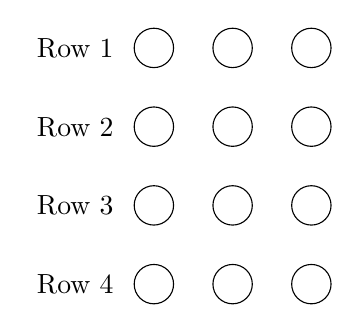
\begin{tikzpicture}
        % Draw the circles and number them
        \foreach \y in {0,1,2,3} {
            \foreach \x in {0,1,2} {
                \node[draw, circle, minimum size=0.5cm] at (\x, -\y) {};
            }
            % Add row numbers
            \node at (-1, -\y) {Row \pgfmathparse{int(\y+1)}\pgfmathresult};
        }
    \end{tikzpicture}
\end{center}

In this grid, we have 4 rows of 3 circles each, which represents $4 \times 3 = 12$.
\begin{itemize}
    \item If you have 4 rows of 3 circles, you can count all the objects (3 + 3 + 3 + 3) or multiply $4 \times 3 = 12$.
\end{itemize}

Let’s try another example:

\textbf{Example:}
\begin{itemize}
    \item How many total buttons do you have if you arrange them in 5 rows with 6 buttons in each row?
    \item Instead of adding 6 five times, multiply: $5 \times 6 = 30$ buttons.
\end{itemize}

\textbf{Try It Yourself:}
\begin{itemize}
    \item How many total apples if you arrange them in 3 rows with 5 apples in each row?
    \item Multiply: $3 \times 5$ = ?
\end{itemize}

\section{What Is Division?}
Division is the reverse of multiplication. It’s used to split a total into equal parts or to see how many times one number can fit into another. For example:
\begin{itemize}
    \item You have 12 candies and want to share them equally among 4 friends. How many candies does each friend get?
\end{itemize}

This is a division problem:
\begin{itemize}
    \item $12 \div 4 = 3$ (Each friend gets 3 candies.)
\end{itemize}

Here’s how it works:
\begin{itemize}
    \item $12 \div 4$ means "How many groups of 4 can I make from 12?"
\end{itemize}

\subsection{Visualizing Division}
We can also use arrays and grouping to understand division. Imagine you have 12 candies, and you want to put them into groups of 4. You would end up with 3 groups of 4, which tells you that $12 \div 4 = 3$.
\begin{center}
    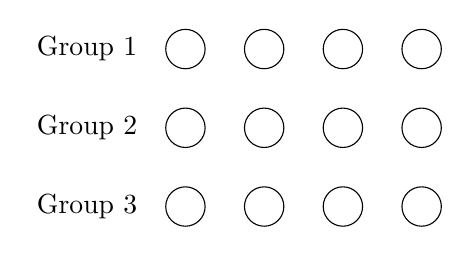
\begin{tikzpicture}
        % Draw the circles and number them
        \foreach \y in {0,1,2} {
            \foreach \x in {0,1,2,3} {
                \node[draw, circle, minimum size=0.5cm] at (\x, -\y) {};
            }
            % Add group numbers
            \node at (-1.25, -\y) {Group \pgfmathparse{int(\y+1)}\pgfmathresult};
        }
    \end{tikzpicture}
\end{center}

In this grid, we have 3 groups of 4 candies each, which represents $12 \div 4 = 3$.

\textbf{Try It Yourself:}
\begin{itemize}
    \item You have 16 cookies and want to divide them among 4 friends. How many cookies does each friend get?
    \item Divide: $16 \div 4$ = ?
\end{itemize}

\section{The Relationship Between Multiplication and Division}
Multiplication and division are opposite operations, and they are closely related. This means if you know how to multiply, you can use that knowledge to help you divide.

For example, if you know that $4 \times 3 = 12$, you also know:
\begin{itemize}
    \item $12 \div 4 = 3$
    \item $12 \div 3 = 4$
\end{itemize}

This is called the inverse relationship between multiplication and division. When you multiply two numbers to get a product, division allows you to work backwards from that product to find one of the original numbers.

\textbf{Example:}
\begin{itemize}
    \item If $7 \times 8 = 56$, then:
    \begin{itemize}
        \item $56 \div 7 = 8$
        \item $56 \div 8 = 7$
    \end{itemize}
\end{itemize}

\section{Practice Makes Perfect: Let’s Try Some Exercises!}
\begin{multicols}{2}
    \subsection{Simple Multiplication:}
    \begin{enumerate}
        \item $3 \times 4 = \underline{\hspace{0.5cm}}$
        \item $5 \times 6 = \underline{\hspace{0.5cm}}$
        \item $8 \times 7 = \underline{\hspace{0.5cm}}$
    \end{enumerate}

    \subsection{Simple Division:}
    \begin{enumerate}
        \item $12 \div 4 = \underline{\hspace{0.5cm}}$
        \item $20 \div 5 = \underline{\hspace{0.5cm}}$
        \item $36 \div 6 = \underline{\hspace{0.5cm}}$
    \end{enumerate}
\end{multicols}
Remember, multiplication is repeated addition, and division is splitting into equal parts. Practice using these operations with real objects, such as grouping items or dividing things equally among friends.

\section{Everyday Examples of Multiplication and Division}
Just like addition and subtraction, multiplication and division show up in everyday life. Let’s look at some examples:
\begin{itemize}
    \item \textbf{Cooking:} If a recipe calls for 3 eggs and you’re doubling the recipe, you’ll multiply: $3 \times 2 = 6$ eggs.
    \item \textbf{Shopping:} You’re buying 5 packs of juice, and each pack has 6 bottles. To find the total number of bottles, multiply: $5 \times 6 = 30$ bottles.
    \item \textbf{Splitting Costs:} You and 3 friends are splitting the cost of a \$40 meal equally. To find out how much each person should pay, divide: $40 \div 4 = 10$.
    \item \textbf{Sports:} You have 12 players and want to create teams of 4. Divide: $12 \div 4 = 3$ teams.
\end{itemize}

\section{The Properties of Multiplication}
Just like with addition, multiplication has some useful properties:

\subsection{Commutative Property of Multiplication:}
\begin{itemize}
    \item The order in which you multiply numbers doesn’t matter.
    \item For example, $3 \times 5$ is the same as $5 \times 3$. Both equal 15.
    \item \textbf{Example:} $2 \times 4 = 8$ and $4 \times 2 = 8$.
\end{itemize}

\subsection{Associative Property of Multiplication:}
\begin{itemize}
    \item When multiplying three or more numbers, the way you group them doesn’t change the result.
    \item For example, $(2 \times 3) \times 4 = 2 \times (3 \times 4)$. Both equal 24.
    \item \textbf{Example:} $(1 \times 2) \times 3 = 1 \times (2 \times 3)$.
\end{itemize}

\subsection{Distributive Property:}
\begin{itemize}
    \item You can break up multiplication over addition.
    \item For example, $4 \times (2 + 3)$ is the same as $(4 \times 2) + (4 \times 3)$. Both equal 20.
    \item \textbf{Example:}$ 3 \times (1 + 2) = (3 \times 1) + (3 \times 2)$.
\end{itemize}

\section{Breaking It Down: Solving Word Problems with Multiplication and Division}
Just like with addition and subtraction, word problems are a great way to see how multiplication and division work in real life.

\textbf{Example 1:} A farmer has 6 apple trees. Each tree produces 10 apples. How many apples does the farmer have in total?
\begin{itemize}
    \item \textbf{Step 1:} Identify what you know.
        The farmer has 6 trees, and each tree produces 10 apples.
    \item \textbf{Step 2:} Write the math problem.
        $6 \times 10 = 60$ apples.
\end{itemize}

\textbf{Example 2:} You have 24 chocolates, and you want to divide them equally among 6 people. How many chocolates does each person get?
\begin{itemize}
    \item \textbf{Step 1:} Identify what you know:
        You have 24 chocolates, and there are 6 people.
    \item \textbf{Step 2:} Write the math problem:
        $24 \div 6 = 4$ chocolates per person.
\end{itemize}

\section{Chapter Summary}
\begin{itemize}
    \item Multiplication is repeated addition, and division is splitting into equal parts.
    \item We can visualize multiplication and division using arrays, groups, and real-world objects.
    \item Multiplication and division are related through the inverse relationship: knowing one helps you solve the other.
    \item You can use multiplication and division in everyday life, such as doubling recipes, splitting costs, or organizing objects.
    \item We learned the commutative, associative, and distributive properties of multiplication.
\end{itemize}

\section{Challenge Question:}
\begin{enumerate}[label=(\alph*)]
    \item You have 18 candies, and you want to put them into bags with 3 candies in each bag. How many bags do you need?
    \begin{itemize}
        \item $18 \div 3 = \underline{\hspace{0.5cm}}$
    \end{itemize}
    \item You have 45 apples, and you want to put them into baskets with 5 apples in each basket. How many baskets do you need?
    \begin{itemize}
        \item $45 \div 5 = \underline{\hspace{0.5cm}}$
    \end{itemize}
    \item A classroom has 30 students, and the teacher wants to divide them into groups of 6. How many groups will there be?
    \begin{itemize}
        \item $30 \div 6 = \underline{\hspace{0.5cm}}$
    \end{itemize}
    \item You have 72 marbles and want to divide them equally among 8 friends. How many marbles does each friend get?
    \begin{itemize}
        \item $72 \div 8 = \underline{\hspace{0.5cm}}$
    \end{itemize}
    \item A baker has 120 cookies and wants to pack them into boxes with 10 cookies each. How many boxes are needed?
    \begin{itemize}
        \item $120 \div 10 = \underline{\hspace{0.5cm}}$
    \end{itemize}
    \item You have 56 pencils and want to distribute them equally into 7 pencil cases. How many pencils will each pencil case contain?
    \begin{itemize}
        \item $56 \div 7 = \underline{\hspace{0.5cm}}$
    \end{itemize}
    \item A gardener has 81 flowers and wants to plant them in rows with 9 flowers each. How many rows will there be?
    \begin{itemize}
        \item $81 \div 9 = \underline{\hspace{0.5cm}}$
    \end{itemize}
    \item You have 64 books and want to arrange them on 8 shelves equally. How many books will each shelf have?
    \begin{itemize}
        \item $64 \div 8 = \underline{\hspace{0.5cm}}$
    \end{itemize}
    \item A factory produces 90 toys and packs them into boxes with 15 toys each. How many boxes are needed?
    \begin{itemize}
        \item $90 \div 15 = \underline{\hspace{0.5cm}}$
    \end{itemize}
    \item You have 99 candies and want to divide them equally among 11 children. How many candies will each child get?
    \begin{itemize}
        \item $99 \div 11 = \underline{\hspace{0.5cm}}$
    \end{itemize}
    \item A farmer has 144 eggs and wants to pack them into cartons with 12 eggs each. How many cartons are needed?
    \begin{itemize}
        \item $144 \div 12 =  \underline{\hspace{0.5cm}}$
    \end{itemize}
\end{enumerate}

\chapter{Fractions, Decimals, and Percentages - Parts of a Whole}

\section{Introduction: Why Learn About Fractions, Decimals, and Percentages?}
In the previous chapters, you learned about whole numbers and how to add, subtract, multiply, and divide them. But not everything in life comes in whole numbers. Sometimes, we need to talk about parts of things. This is where fractions, decimals, and percentages come in. Whether you’re measuring ingredients in a recipe, calculating a sale discount, or sharing a pizza with friends, you’re dealing with parts of a whole. These concepts are essential in daily life and will help you tackle more complex math problems down the road.

\section{What Is a Fraction?}
A fraction is a way to represent parts of a whole. It’s made up of two parts: the numerator (the top number), which tells you how many parts you have, and the denominator (the bottom number), which tells you how many equal parts the whole is divided into. For example:
\begin{itemize}
    \item In the fraction $\frac{1}{2}$, the numerator is 1, and the denominator is 2. This means we have 1 part out of 2 equal parts, or "one-half."
    \item In the fraction $\frac{3}{4}$, the numerator is 3, and the denominator is 4. This means we have 3 parts out of 4 equal parts, or "three-quarters."
\end{itemize}

\subsection{Visualizing Fractions}
You can picture fractions by thinking of a pie or pizza. Imagine cutting a pizza into 4 equal slices. Each slice is $\frac{1}{4}$ of the pizza. If you eat 2 slices, you’ve eaten 2 out of 4 parts, or $\frac{2}{4}$ of the pizza (which simplifies to $\frac{1}{2}$).

\begin{center}
    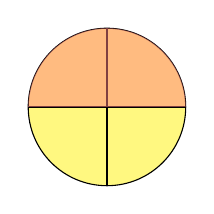
\begin{tikzpicture}
        % Draw the pizza
        \filldraw[fill=yellow!50] (0,0) circle (1);
        % Draw the slices
        \draw (0,0) -- (0:0);
        \draw (0,0) -- (90:1);
        \draw (0,0) -- (180:1);
        \draw (0,0) -- (270:1);
        \draw (0,0) -- (360:1);
        % Shade the eaten slices
        \fill[red!50, opacity=0.5] (0,0) -- (0:1) arc (0:180:1) -- cycle;
    \end{tikzpicture}
    \end{center}

\subsection{Key Vocabulary}
\begin{itemize}
    \item \textbf{Proper fraction:} The numerator is smaller than the denominator (e.g., $\frac{3}{4}$).
    \item \textbf{Improper fraction:} The numerator is greater than or equal to the denominator (e.g., $\frac{5}{4}$).
    \item \textbf{Mixed number:} A whole number combined with a fraction (e.g., $1 \frac{1}{2}$).
\end{itemize}

\section{What Is a Decimal?}
A decimal is another way to represent parts of a whole, especially when working with the base-10 number system. Decimals are often used in money, measurements, and scientific data.

\subsection{Understanding Place Value in Decimals}
Just as whole numbers have place values (ones, tens, hundreds, etc.), decimals have place values for parts smaller than one:
\begin{itemize}
    \item 0.1 is one-tenth.
    \item 0.01 is one-hundredth.
    \item 0.001 is one-thousandth.
\end{itemize}

For example:
\begin{itemize}
    \item 0.5 means 5 tenths (or $\frac{1}{2}$), so it’s half of 1.
    \item 0.75 means 75 hundredths (or $\frac{3}{4}$), so it’s three-quarters of 1.
\end{itemize}

\subsection{Converting Fractions to Decimals}
We can convert fractions to decimals by dividing the numerator by the denominator. For example:
\begin{itemize}
    \item $\frac{1}{2} = 1 \div 2 = 0.5$
    \item $\frac{3}{4} = 3 \div 4 = 0.75$
\end{itemize}

\section{What Is a Percentage?}
A percentage is a way to describe parts of a whole using 100 as the reference point. It’s essentially a fraction out of 100. Percentages are extremely useful in everyday life, especially for things like discounts, taxes, and grades.

\subsection{Understanding Percentages}
\begin{itemize}
    \item 50\% means 50 out of 100, or half.
    \item 25\% means 25 out of 100, or one-quarter.
    \item 100\% means the whole thing.
\end{itemize}

\subsection{Converting Percentages to Fractions and Decimals}
\begin{itemize}
    \item 50\% = $\frac{50}{100}$ = $\frac{1}{2}$ = 0.5
    \item 25\% = $\frac{25}{100}$ = $\frac{1}{4}$ = 0.25
    \item 75\% = $\frac{75}{100}$ = $\frac{3}{4}$ = 0.75
\end{itemize}

You can also convert fractions and decimals into percentages:
\begin{itemize}
    \item $\frac{1}{2}$ = 0.5 = 50\%
    \item $\frac{3}{4}$ = 0.75 = 75\%
\end{itemize}

To convert a decimal to a percentage, multiply by 100. For example:
\begin{enumerate}
    \item $0.2 \times 100$ = 20\%
    \item $0.65 \times 100$ = 65\% 
\end{enumerate}

\section{How to Work with Fractions}
\subsection{Adding and Subtracting Fractions}
When adding or subtracting fractions, they must have the same denominator (the bottom number). Example:
\begin{itemize}
    \item $\frac{1}{3} + \frac{2}{3} = ?$ The denominators are the same, so we add the numerators: 1 + 2 = 3. The answer is $\frac{3}{3}$, which simplifies to 1.
    \item $\frac{3}{4} - \frac{1}{2} = ?$ First, find a common denominator. For $\frac{3}{4}$ and $\frac{1}{2}$, the least common denominator is 4. Convert $\frac{1}{2}$ to $\frac{2}{4}$, so now you have: $\frac{3}{4} - \frac{2}{4} = \frac{1}{4}$.
\end{itemize}

\subsection{Multiplying and Dividing Fractions}
When multiplying fractions, simply multiply the numerators and then the denominators. Example:
\begin{itemize}
    \item $\frac{1}{2} \times \frac{2}{3} = ?$ Multiply the numerators: $1 \times 2 = 2$. Multiply the denominators: $2 \times 3 = 6$. The answer is $\frac{2}{6}$, which simplifies to $\frac{1}{3}$.
\end{itemize}

When dividing fractions, multiply by the reciprocal of the second fraction (flip the numerator and denominator). Example:
\begin{itemize}
    \item $\frac{1}{2} \div \frac{2}{3} = ?$ Flip the second fraction to get $\frac{3}{2}$, and then multiply: $\frac{1}{2} \times \frac{3}{2} = \frac{3}{4}$.
\end{itemize}

\section{How to Work with Decimals}
\subsection{Adding and Subtracting Decimals}
To add or subtract decimals, make sure the decimal points are lined up. Example:
\begin{itemize}
    \item $3.25 + 1.1 = ?$ Line up the decimal points: $3.25 + 1.10 = 4.35$.
\end{itemize}

\subsection{Multiplying Decimals}
Multiply as if there were no decimal points, then count the total number of decimal places in the factors to place the decimal in the product. Example:
\begin{itemize}
    \item $0.25 \times 0.5 = ?$ Multiply $25 \times 5 = 125$. Count the decimal places: 2 in 0.25 and 1 in 0.5 (so 3 decimal places total). The answer is 0.125.
    \item $1.2 \times 2 = ?$ Multiply $12 \times 2 = 24$. There is 1 decimal place in 1.2, so the answer is 2.4.
\end{itemize}

\subsection{Dividing Decimals}
Move the decimal point in the divisor (the number you're dividing by) to make it a whole number, and move the decimal point in the dividend (the number you're dividing) the same number of places. Example:
\begin{itemize}
    \item $0.6 \div 0.2 = ?$ Move the decimal in 0.2 one place to the right (to make it 2). Move the decimal in 0.6 one place to the right (to make it 6). Now divide: $6 \div 2 = 3$.
    \item $0.75 \div 0.25 = ?$ Move the decimal in 0.25 two places to the right (to make it 25). Move the decimal in 0.75 two places to the right (to make it 75). Now divide: $75 \div 25 = 3$.
\end{itemize}

\section{How to Work with Percentages}
\subsection{Finding a Percentage of a Number}
To find a percentage of a number, multiply the number by the percentage as a decimal. Example:
\begin{itemize}
    \item $20\% of 50 = ?$ Convert 20\% to a decimal (0.20), then multiply: $50 \times 0.20 = 10$.
\end{itemize}

\subsection{Converting a Number to a Percentage}
To convert a number to a percentage, multiply it by 100 and add the \% symbol. Example:
\begin{itemize}
    \item $0.75 = ?$ Multiply: $0.75 \times 100 = 75\%$. So, 0.75 is 75\%.
\end{itemize}

\section{Practice Makes Perfect: Let’s Try Some Exercises!}
\subsection{Fractions}
\begin{enumerate}
    \item $\frac{2}{3} + \frac{1}{3} = \_\_\_\_$
    \item $\frac{3}{4} - \frac{1}{4} = \_\_\_\_$
    \item $\frac{1}{2} \times \frac{2}{3} = \_\_\_\_$
\end{enumerate}

\subsection{Decimals}
\begin{enumerate}
    \item $1.2 + 0.8 = \_\_\_\_$
    \item $5.5 \div 2.5 = \_\_\_\_$
    \item $0.25 \times 0.4 = \_\_\_\_$
\end{enumerate}

\subsection{Percentages}
\begin{enumerate}
    \item 25\% of 80 = \_\_\_\_
    \item Convert 0.6 to a percentage = \_\_\_\_
    \item Convert $\frac{1}{5}$ to a percentage = \_\_\_\_
\end{enumerate}

\section{Real-Life Applications of Fractions, Decimals, and Percentages}
\subsection{Cooking}
Recipes often use fractions (e.g., $\frac{1}{2}$ cup of sugar). If you’re doubling the recipe, you need to multiply those fractions.

\subsection{Shopping}
You see a 30\% discount on an item. To find the sale price, you need to calculate 30\% of the original price.

\subsection{Money}
If you earn \$50 and save 20\%, how much money are you saving? Find 20\% of \$50 to see that you’re saving \$10.

\section{Converting Between Fractions, Decimals, and Percentages}
Understanding how to convert between fractions, decimals, and percentages is essential. These forms all represent parts of a whole, but they are useful in different situations. Let's explore how to move between these forms.

\subsection{Converting Fractions to Decimals}
To convert a fraction to a decimal, divide the numerator (top number) by the denominator (bottom number). Example:
\begin{itemize}
    \item Convert $\frac{3}{4}$ to a decimal: $\frac{3}{4} = 3 \div 4 = 0.75$
    \item Convert $\frac{1}{2}$ to a decimal: $\frac{1}{2} = 1 \div 2 = 0.5$
\end{itemize}

\subsection{Converting Decimals to Fractions}
To convert a decimal to a fraction, write the decimal as the numerator and use the place value of the decimal as the denominator. Example:
\begin{itemize}
    \item Convert 0.25 to a fraction: $0.25 = \frac{25}{100}$, which simplifies to $\frac{1}{4}$
    \item Convert 0.6 to a fraction: $0.6 = \frac{6}{10}$, which simplifies to $\frac{3}{5}$
\end{itemize}

\subsection{Converting Fractions to Percentages}
To convert a fraction to a percentage, first divide the numerator by the denominator to get a decimal. Then, multiply the decimal by 100 to find the percentage. Example:
\begin{itemize}
    \item Convert $\frac{3}{5}$ to a percentage: $\frac{3}{5} = 3 \div 5 = 0.6$ $0.6 \times 100 = 60\%$
    \item Convert $\frac{7}{8}$ to a percentage: $\frac{7}{8} = 7 \div 8 = 0.875$ $0.875 \times 100 = 87.5\%$
\end{itemize}

\subsection{Converting Percentages to Fractions}
To convert a percentage to a fraction, write the percentage as the numerator and 100 as the denominator, then simplify if possible. Example:
\begin{itemize}
    \item Convert 75\% to a fraction: $75\% = \frac{75}{100}$, which simplifies to $\frac{3}{4}$
    \item Convert 20\% to a fraction: $20\% = \frac{20}{100}$, which simplifies to $\frac{1}{5}$
\end{itemize}

\subsection{Converting Decimals to Percentages}
To convert a decimal to a percentage, multiply the decimal by 100 and add the \% sign. Example:
\begin{itemize}
    \item Convert 0.85 to a percentage: $0.85 \times 100 = 85\%$
    \item Convert 0.125 to a percentage: $0.125 \times 100 = 12.5\%$
\end{itemize}

\subsection{Converting Percentages to Decimals}
To convert a percentage to a decimal, divide by 100 or move the decimal point two places to the left. Example:
\begin{itemize}
    \item Convert 50\% to a decimal: $50 \div 100 = 0.50$
    \item Convert 12.5\% to a decimal: $12.5 \div 100 = 0.125$
\end{itemize}

\section{Real-Life Applications of Fractions, Decimals, and Percentages}
Fractions, decimals, and percentages are not just theoretical concepts; they show up frequently in everyday situations. Let’s explore some practical applications:

\subsection{Shopping and Discounts}
When you're shopping, discounts are often given as percentages. If a shirt is 25\% off, how do you know how much you're saving? Example:
\begin{itemize}
    \item The original price of the shirt is \$40, and it’s 25\% off. First, convert 25\% to a decimal: $25\% = 0.25$ Multiply the price by the discount: $40 \times 0.25 = 10$ You are saving \$10, so the new price is $\$40 - 10 = 30$.
\end{itemize}

\subsection{Cooking}
Recipes often require you to use fractions when measuring ingredients, such as $\frac{1}{2}$ cup of flour or $\frac{1}{4}$ teaspoon of salt. Example:
\begin{itemize}
    \item If a recipe calls for $\frac{1}{2}$ cup of sugar and you want to double the recipe, you’ll need to multiply the fraction by 2: $\frac{1}{2} \times 2 = 1$ cup of sugar.
\end{itemize}

\subsection{Time}
Fractions and percentages are also used in managing time. For example, if you work for 8 hours and spend 3 hours in meetings, what fraction of your time was spent in meetings? Example:
\begin{itemize}
    \item $\frac{3}{8}$ of your workday was spent in meetings.
\end{itemize}

\subsection{Grades}
Grades are often represented as percentages. If you scored 18 out of 20 on a test, what percentage is that? Example:
\begin{itemize}
    \item $\frac{18}{20} = 0.9$, and $0.9 \times 100 = 90\%$
\end{itemize}

\section{Practice Makes Perfect: Let’s Try Some Exercises!}
\subsection{Converting Between Forms}
\begin{itemize}
    \item Convert $\frac{3}{8}$ to a decimal.
    \item Convert 0.75 to a fraction.
    \item Convert 45\% to a fraction and simplify.
    \item Convert $\frac{7}{10}$ to a percentage.
\end{itemize}

\subsection{Word Problems}
\begin{itemize}
    \item A store is having a sale, and all items are 30\% off. If the original price of a pair of shoes is \$60, how much will the shoes cost after the discount?
    \item You spent $\frac{1}{4}$ of your day exercising. What percentage of your day did you spend exercising?
    \item In a class of 25 students, 15 are wearing blue shirts. What percentage of the class is wearing blue shirts?
\end{itemize}

\section{Chapter Summary}
Fractions represent parts of a whole, and you can add, subtract, multiply, and divide them just like whole numbers.
Decimals are another way to express parts of a whole, especially when working in the base-10 system. You can perform arithmetic operations with decimals just as you do with whole numbers.
Percentages represent parts of a whole in terms of 100 and are useful in many real-life applications such as discounts, grades, and statistics.
Converting between fractions, decimals, and percentages is an essential skill for understanding and comparing parts of a whole in different forms.

\subsection{Challenge Question}
You bought a sweater for \$48 after a 20\% discount. What was the original price of the sweater? (Hint: If you received a 20\% discount, you paid 80\% of the original price.)

This chapter builds a bridge between fractions, decimals, and percentages, making them easier to understand and apply in real-world scenarios. As you continue practicing, you'll become more comfortable converting between these forms and using them to solve everyday problems. Keep practicing, and these concepts will become second nature!
\chapter{Patterns and Relationships – Introduction to Algebra}
\section{Introduction: The Power of Variables and Equations}
In the previous chapters, we explored numbers, addition, subtraction, multiplication, devision, fractions, decimals, and percentages. Now, we are ready to enter the world of algebra. Algebra may seem intimidating at first, but it's simply a way of using letters and symbols to represent numbers and relationships between them.

Why is algebra important? Because it allows us to solve problems where we don't know all the information yet. Whether you're calculating the price of multiple items, planning how to save money, or figuring out how far you've traveled, algebra helps you break these problems down and find solutions.

\section{What Is a Variable?}
A variable is a symbol (often a letter) that represents a number we don’t know yet. Think of it as a blank space that will eventually be filled in.

For example:

If you don’t know how many apples you have, you can use $x$ to represent the number of apples.
Here’s how it looks:

\begin{quote}
"I have $x$ apples."
\end{quote}

Using Variables in Equations: You can use variables to create equations, which are like math sentences that describe relationships between numbers.

For example:

You buy 3 apples, and you already had $x$ apples. The equation would look like this:
\[ x + 3 \]
(This means "the number of apples I already had plus 3 more apples.")

\section{What Is an Equation?}
An equation is a statement that two things are equal. It has two sides, usually with an equal sign (=) in the middle.

Here’s an example:

\[ x + 3 = 7 \]
This equation says that if you add 3 to some unknown number $x$, you will get 7.

Your job using algebra is often to solve the equation—to figure out what number $x$ represents.

\section{Solving Simple Equations}
The key to solving equations is to isolate the variable on one side of the equation. Let’s go back to the equation $x + 3 = 7$.

\begin{enumerate}
    \item Subtract 3 from both sides.
    \begin{quote}
    Why? Because you want to get $x$ by itself.
    \[ x + 3 - 3 = 7 - 3 \]
    \end{quote}
    \item Simplify.
    \[ x = 4 \]
\end{enumerate}

Now, we know that $x$ equals 4. This means you originally had 4 apples before buying 3 more.

\section{Understanding Patterns and Relationships}
Algebra is also about recognizing patterns and relationships between numbers. For example, if you know that the number of apples increases by 3 every day, you could describe this pattern with an equation.

Let’s say:

\begin{itemize}
    \item $x$ represents the number of apples you have.
    \item $d$ represents the number of days.
\end{itemize}

Each day, you get 3 more apples, so you can write:

\[ x = 3d \]
This equation shows that the number of apples ($x$) is equal to 3 times the number of days ($d$).
\begin{quote}
    Let $d = 5$ (the number of days).
    Then, using the equation $x = 3d$:
    \[ x = 3 \times 5 \]
    \[ x = 15 \]
\end{quote}

\section{Working with Word Problems in Algebra}
Let’s take a word problem and see how algebra helps us solve it:

\textbf{Problem:} Sarah has 5 books, and she buys 2 more books each week. How many books will Sarah have after 4 weeks?

\begin{enumerate}
    \item Identify what you know.
    \begin{itemize}
        \item Sarah starts with 5 books.
        \item She buys 2 more books every week.
        \item The number of weeks is 4.
    \end{itemize}
    \item Write the equation.
    \begin{quote}
    Let $x$ represent the number of books after 4 weeks.
    The total number of books is the 5 she started with, plus 2 books for each week:
    \[ x = 5 + 2 \times 4 \]
    \end{quote}
    \item Solve the equation.
    \[ x = 5 + 8 \]
    \[ x = 13 \]
\end{enumerate}

So, after 4 weeks, Sarah will have 13 books.

\section{The Distributive Property in Algebra}
In algebra, you’ll often come across expressions that use parentheses. When this happens, you can use the distributive property to simplify the expression.

The distributive property says:

\[ a(b + c) = ab + ac \]

For example:

\[ 2(3 + 4) \]
Using the distributive property, we can multiply 2 by both 3 and 4:
\[ 2(3 + 4) = 2 \times 3 + 2 \times 4 \]
\[ = 6 + 8 \]
\[ = 14 \]
This is helpful when solving more complex equations.

\section{Combining Like Terms}
Sometimes in algebra, you'll have similar terms that can be combined. These are called like terms. Like terms have the same variable raised to the same power.

Example:

\[ 3x + 4x \]
Both terms have the variable $x$, so you can add them together:
\[ 3x + 4x = 7x \]
This makes the equation simpler and easier to work with.

\section{Practice Makes Perfect: Let’s Try Some Exercises!}
\textbf{Solving Simple Equations:}
\begin{itemize}
    \item $x + 5 = 12$
    \item $y - 3 = 9$
    \item $2x = 10$
\end{itemize}

\textbf{Writing Algebraic Expressions:}
\begin{itemize}
    \item Write an expression for "5 more than a number $n$."
    \item Write an equation for "A number $y$ divided by 2 equals 6."
\end{itemize}

\textbf{Word Problems:}
\begin{itemize}
    \item John has 10 marbles. He buys 3 more marbles every day. How many marbles will he have after 5 days?
    \item Maria has twice as many apples as her friend. If her friend has $x$ apples, how many apples does Maria have?
\end{itemize}

\section{Real-Life Applications of Algebra}
\begin{itemize}
    \item \textbf{Budgeting:} If you have a fixed income every month and certain expenses, you can use algebra to figure out how much money you'll have left.
    \item \textbf{Travel:} If you’re driving at a certain speed, you can use algebra to calculate how long it will take you to reach your destination.
    \item \textbf{Shopping:} If you know the price of one item, you can use algebra to calculate the total cost for several of the same item.
\end{itemize}

\section{Chapter Summary}
\begin{itemize}
    \item A variable is a letter that represents an unknown number.
    \item An equation is a statement that two things are equal.
    \item You can solve equations by isolating the variable.
    \item Algebra is about recognizing patterns and relationships between numbers.
    \item The distributive property helps you simplify expressions with parentheses.
    \item You can combine like terms to make equations simpler.
\end{itemize}

Algebra allows you to explore the relationships between numbers in a more abstract way, and it will continue to be an essential tool as you progress to more advanced math topics like geometry and functions.

\section{Challenge Questions:}
\begin{enumerate}[label=(\alph*)]
    \item You’re at a store, and the total cost of your items is $x$. You give the cashier \$20, and you get \$4 in change. Write an equation to represent this situation, and solve for $x$ (the total cost of your items).
    \item A rectangle has a length of $l$ and a width of $w$. The perimeter of the rectangle is 20 units. Write an equation to represent this situation, and solve for $l$ if $w = 4$ units.
    \item The sum of three consecutive integers is 45. Write an equation to represent this situation, and solve for the integers.
    \item A car travels at a speed of $s$ miles per hour. If the car travels for 3 hours, the total distance covered is 150 miles. Write an equation to represent this situation, and solve for $s$.
    \item The area of a triangle is 24 square units. The base of the triangle is $b$ units, and the height is $h$ units. Write an equation to represent this situation, and solve for $h$ if $b = 8$ units.
    \item A number $n$ is increased by 5 and then multiplied by 2 to give a result of 18. Write an equation to represent this situation, and solve for $n$.
    \item The difference between two numbers is 7. If the larger number is $x$ and the smaller number is $y$, write an equation to represent this situation, and solve for $x$ if $y = 5$.
    \item The product of a number $p$ and 4 is equal to 32. Write an equation to represent this situation, and solve for $p$.
    \item A person has $d$ dollars. After spending \$35, they have \$25 left. Write an equation to represent this situation, and solve for $d$.
    \item The sum of twice a number $m$ and 3 is equal to 17. Write an equation to represent this situation, and solve for $m$.
\end{enumerate}
\chapter{The Power of Geometry – Shapes, Spaces, and Measurement}

\section{Introduction: Why Geometry Matters}
Geometry is all around us. Every building, park, or road we see has some geometric form. When you arrange furniture in a room, measure the length of a wall, or even look at patterns in nature, you're interacting with geometric concepts.

Geometry helps us understand the properties of shapes and spaces, and how to measure and compare them. It’s one of the oldest branches of math, yet it remains one of the most practical.

In this chapter, we’ll explore the basics of geometry, focusing on shapes, angles, areas, and volumes, and how to apply these concepts in real-life situations.

\section{Basic Geometric Shapes and Their Properties}
Let’s start by getting familiar with the most common geometric ideas. Points are like the dot on a number line it has not length, widght or hight. Next we can think of a line of a set of continuous points. This line continues on in both directions to infinity. In Euclidean geometry, an angle is the figure formed by two rays, called the sides of the angle, sharing a common endpoint, called the vertex of the angle. Now lets consider 2D shapes (two-dimensional, flat shapes) and 3D shapes (three-dimensional, solid shapes).

\subsection{\textbf{Notation:}}
We use certain symbols and terms to describe geometric shapes and concepts. Here are some common ones:
\begin{table}[h!]
    \centering
    \begin{tabular}{|c|l|}
        \hline
        \textbf{Symbol} & \textbf{Meaning} \\ \hline
        $\alpha, \beta, \gamma$ & Angles \\ \hline
        $A, B, C$ & Vertices of a triangle \\ \hline
        $a, b, c$ & Sides of a triangle and the side of a square \\ \hline
        $r$ & Radius of a circle \\ \hline
        $h$ & Height of a triangle or the height of a cylinder \\ \hline
        $l$ & Length of a rectangle or the length of a rectangular prism \\ \hline
        $w$ & Width of a rectangle or the width of a rectangular prism \\ \hline
        $s$ & Side of a cube \\ \hline
        $d$ & Diameter of a circle \\ \hline
        $V$ & Volume of a 3D shape \\ \hline
        $P$ & Perimeter of a 2D shape \\ \hline
        $A$ & Area of a 2D shape \\ \hline
        $\pi$ & The constant pi, approximately 3.14159 \\ \hline
    \end{tabular}
    \caption{Notation used in Geometry}
    \label{tab:notation}
\end{table}

\subsection{Point}
A point represents a location in space. It has no length, width, or height.
We can represent a point visually as a dot on a coordinate plane:
\[
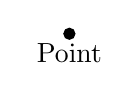
\begin{tikzpicture}
    \filldraw (0,0) circle (2pt);
    \node[below] at (0,0) {Point};
\end{tikzpicture}
\]

\subsection{Lines}
A line is a set of continuous points that extends infinitely in both directions. It has no thickness.
\[
\begin{tikzpicture}
    \draw (-2,0) -- (2,0);
    \node[below] at (0,0) {Line};
\end{tikzpicture}
\]

\subsection{Angle}
An angle is formed when two lines meet at a point. The size of an angle is measured in degrees. The degrees are notated with a small circle in the upper right corner of the number. Minutes and seconds are noted as follows: one degree is divided into 60 minutes (notated with a single quote, e.g., \(45^\circ 30'\)), and one minute is divided into 60 seconds (notated with a double quote, e.g., \(45^\circ 30' 15''\)).

\[
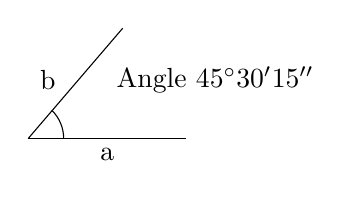
\begin{tikzpicture}
    % Draw the base line
    \draw (0,0) -- (2,0);
    \node[below] at (1,0) {a};
    % Draw the second line
    \draw (0,0) -- (1.2,1.4);
    \node[above] at (0.25,0.5) {b};
    % Add the angle label
    \node[right] at (1,0.75) {Angle \(45^\circ 30' 15''\)};
    % Draw the arc representing the angle
    \draw (0.45,0) arc[start angle=0, end angle=45.5042, radius=0.5];
\end{tikzpicture}
\]

\subsubsection{Types of Angles}
\begin{itemize}
    \item Acute Angle: Less than 90 degrees.
    \item Right Angle: Exactly 90 degrees.
    \item Obtuse Angle: Greater than 90 degrees but less than 180 degrees.
\end{itemize}

\[
\begin{tikzpicture}
    % Acute angle
    \draw[thick,->] (0,0) -- (2,0);
    \draw[thick,->] (0,0) -- (1.5,1) node[above] {Acute};
    \draw[red,thick] (0.5,0) arc[start angle=0, end angle=30, radius=0.5];

    % Right angle
    \draw[thick,->] (5,0) -- (7,0);
    \draw[thick,->] (5,0) -- (5,2) node[above] {Right};
    \draw (5.2,0) -- (5.2,0.2) -- (5,0.2);

    % Obtuse angle
    \draw[thick,->] (10,0) -- (12,0);
    \draw[thick,->] (10,0) -- (11,2) node[above] {Obtuse};
    \draw[red,thick] (10.5,0) arc[start angle=0, end angle=120, radius=0.5];
\end{tikzpicture}
\]

\subsection{Right Angle}
A right angle measures exactly 90 degrees. It looks like the corner of a square.
\textbf{Note:} The symbol for a right angle is a small square in the corner of the angle.
\[
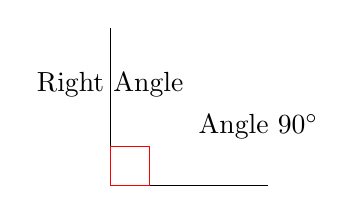
\begin{tikzpicture}
    % Draw the base line
    \draw (0,0) -- (2,0);
    \draw (0,0) -- (0,2);
    % Add the angle label
    \node[right] at (1,0.75) {Angle \(90^\circ\)};
    \node[above] at (0,1) {Right Angle};
    % Draw the square symbol for a right angle
    \draw[red] (0,0) rectangle (0.5,0.5);
\end{tikzpicture}
\]

\subsection{2D Shapes}
\subsubsection{Square}
\begin{itemize}
    \item All four sides are equal in length.
    \item Each angle is 90 degrees (a right angle).
    \item A is the length and hight of the square.
\end{itemize}

\[
\begin{tikzpicture}
    % Draw a square
    \draw (0,0) rectangle (2,2);

    % Draw right angle symbols inside the square
    \node (A) at (-.5,1) {A};
    \draw[red] (0,0) rectangle (0.5,0.5);
    \node (A) at (2.5,1) {A};
    \draw[red] (1.5,0) rectangle (2,0.5);
    \node (B) at (1,-.5) {A};
    \draw[red] (0,1.5) rectangle (0.5,2);
    \node (C) at (1,2.5) {A};
    \draw[red] (1.5,1.5) rectangle (2,2);

    % Add a label below the square
    \node[left] at (1.7,1) {Square};
\end{tikzpicture}
\]

\subsubsection{Rectangle}
\begin{itemize}
    \item Opposite sides are equal in length.
    \item Each angle is 90 degrees.
    \item A hight and B width of the rectangle.
\end{itemize}

\[
\begin{tikzpicture}
    \draw (0,0) -- (4,0) -- (4,2) -- (0,2) -- cycle;
    \node[below] at (2,1.25) {Rectangle};
    % Draw right angle symbols inside the square
    \node (A) at (-.5,1) {A};
    \draw[red] (0,0) rectangle (0.5,0.5);
    \node (A) at (4.5,1) {A};
    \draw[red] (3.5,0) rectangle (4,0.5);
    \node (B) at (2,-.5) {B};
    \draw[red] (0,1.5) rectangle (0.5,2);
    \node (C) at (2,2.5) {B};   
    \draw[red] (3.5,1.5) rectangle (4,2);
\end{tikzpicture}
\]
\subsubsection{Triangle}
\begin{itemize}
    \item A shape with three sides.
    \item The sum of the angles inside any triangle is always 180 degrees.
\end{itemize}
\[
\begin{tikzpicture}
    \draw (0,0) -- (2,4) -- (4,0) -- cycle;
    \node[below] at (2,0) {Triangle};
    \node[below left] at (0,0) {$A$};
    \node[above] at (2,4) {$B$};
    \node[below right] at (4,0) {$C$};
    \node[below left] at (1,2) {$\alpha$};
    \node[below right] at (3,2) {$\beta$};
    \node[above] at (2,1) {$\gamma$};
\end{tikzpicture}
\]

\[ 
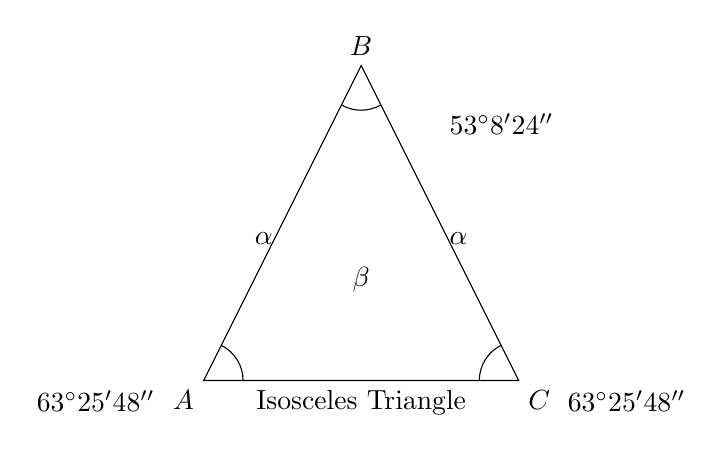
\begin{tikzpicture}
    \draw (0,0) -- (2,4) -- (4,0) -- cycle;
    \node[below] at (2,0) {Isosceles Triangle};
    \node[below left] at (0,0) {$A$};
    \node[above] at (2,4) {$B$};
    \node[below right] at (4,0) {$C$};
    \node[below left] at (1,2) {$\alpha$};
    \node[below right] at (3,2) {$\alpha$};
    \node[above] at (2,1) {$\beta$};
    \draw (.5,0) arc[start angle=0, end angle=63.43, radius=0.5];
    \draw (3.5,0) arc[start angle=180, end angle=116.57, radius=0.5];
    \draw (1.75,3.5) arc[start angle=240, end angle=300, radius=0.5];
    \node[above right] at (3,3) {\(53^\circ 8' 24''\)};
    \node[below left] at (-0.5,0) {\(63^\circ 25' 48''\)};
    \node[below right] at (4.5,0) {\(63^\circ 25' 48''\)};
\end{tikzpicture}
\]

\subsubsection{Equilateral Triangle}
\begin{itemize}
    \item A triangle with all sides of equal length.
    \item All angles are equal.
    \item Each angle measures 60 degrees.
    \item The sum of the angles inside any triangle is always 180 degrees.
    \item The sum of the angles inside an equilateral triangle is always 180 degrees.
\end{itemize}

\[
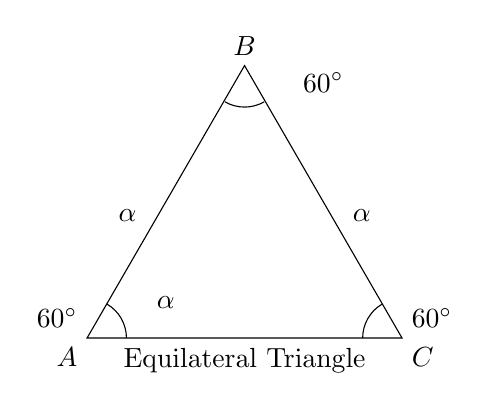
\begin{tikzpicture}
    \draw (0,0) -- (2,3.46) -- (4,0) -- cycle;
    \node[below] at (2,0) {Equilateral Triangle};
    \node[below left] at (0,0) {$A$};
    \node[above] at (2,3.46) {$B$};
    \node[below right] at (4,0) {$C$};
    \node[below left] at (.75,1.75) {$\alpha$};
    \node[below right] at (3.25,1.75) {$\alpha$};
    \node[above] at (,0.25) {$\alpha$};
    \node[below left] at (0,0.5) {$60^\circ$};
    \node[below right] at (4,0.5) {$60^\circ$};
    \node[above] at (3,3) {$60^\circ$};
    \draw (0.5,0) arc[start angle=0, end angle=60, radius=0.5];
    \draw (3.5,0) arc[start angle=180, end angle=120, radius=0.5];
    \draw (1.75,3) arc[start angle=240, end angle=300, radius=0.5];
\end{tikzpicture}
\]

\subsubsection{Scalene Triangle}
\begin{itemize}
    \item A triangle with all sides of different lengths.
    \item All angles are different.
\end{itemize}

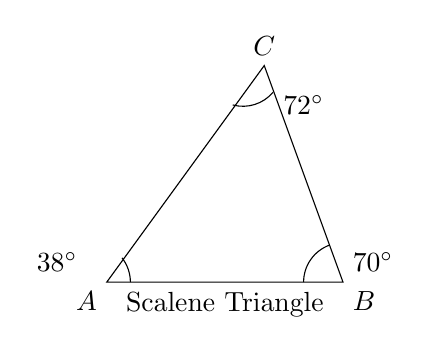
\begin{tikzpicture}
    \draw (0,0) -- (3,0) -- (2,2.75) -- cycle;
    \node[below] at (1.5,0) {Scalene Triangle};
    \node[below left] at (0,0) {$A$};
    \node[below right] at (3,0) {$B$};
    \node[above] at (2,2.75) {$C$};
    \node[below left] at (-0.25,0.5) {$38^\circ$};
    \node[below right] at (3,0.5) {$70^\circ$};
    \node[above] at (2.5,2) {$72^\circ$};
    \draw (0.3,0) arc[start angle=0, end angle=38, radius=0.5];
    \draw (2.5,0) arc[start angle=180, end angle=110, radius=0.5];
    \draw (1.6,2.25) arc[start angle=255, end angle=320, radius=0.5];
\end{tikzpicture}

\subsubsection{Circle}
\begin{itemize}
    \item A round shape where every point on the boundary is the same distance from the center.
    \item The distance from the center to the edge is called the radius.
    \item The total distance around the circle is called the circumference.
\end{itemize}
\[
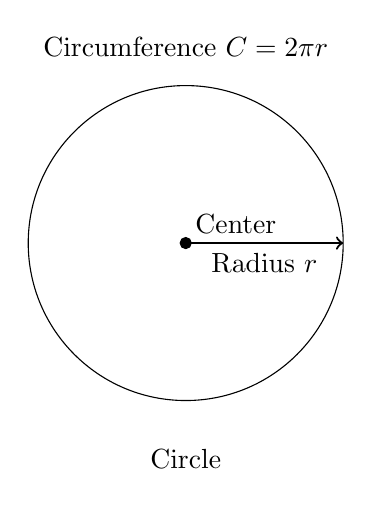
\begin{tikzpicture}
    % Draw the circle with radius 2
    \draw (0,0) circle (2);
    
    % Draw the radius
    \draw[->, thick] (0,0) -- (2,0);
    \node[below] at (1,0) {Radius \(r\)};
    
    % Draw the center point
    \filldraw[black] (0,0) circle (2pt) node[above right] {Center};

    % Draw the circumference label
    \node[above] at (0,2.25) {Circumference \(C = 2\pi r\)};
    
    % Add a label below the circle
    \node[below] at (0,-2.5) {Circle};
\end{tikzpicture}
\]



\subsection{3D Shapes}

\subsubsection{Cube}
\begin{itemize}
    \item All edges are equal, and it has 6 square faces.
\end{itemize}
\[
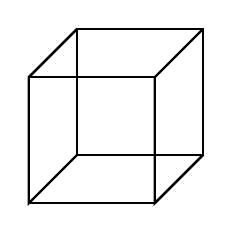
\begin{tikzpicture}[scale=0.8]
    % Draw the cube
    \draw[thick] (0,0,0) -- (2,0,0) -- (2,2,0) -- (0,2,0) -- cycle; % front face
    \draw[thick] (0,0,0) -- (0,0,2) -- (0,2,2) -- (0,2,0); % left face
    \draw[thick] (2,0,0) -- (2,0,2) -- (2,2,2) -- (2,2,0); % right face
    \draw[thick] (0,0,2) -- (2,0,2) -- (2,2,2) -- (0,2,2) -- cycle; % back face
    \draw[thick] (0,2,0) -- (0,2,2); % top-left edge
    \draw[thick] (2,0,0) -- (2,0,2); % bottom-right edge
\end{tikzpicture}
\]

\subsubsection{Rectangular Prism}
\begin{itemize}
    \item Like a cube, but with rectangular faces instead of square ones.
\end{itemize}
\[
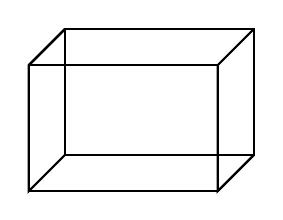
\begin{tikzpicture}[scale=0.8]
    % Draw the rectangular prism
    \draw[thick] (0,0,0) -- (3,0,0) -- (3,2,0) -- (0,2,0) -- cycle; % front face
    \draw[thick] (0,0,0) -- (0,0,1.5) -- (0,2,1.5) -- (0,2,0); % left face
    \draw[thick] (3,0,0) -- (3,0,1.5) -- (3,2,1.5) -- (3,2,0); % right face
    \draw[thick] (0,0,1.5) -- (3,0,1.5) -- (3,2,1.5) -- (0,2,1.5) -- cycle; % back face
    \draw[thick] (0,2,0) -- (0,2,1.5); % top-left edge
    \draw[thick] (3,0,0) -- (3,0,1.5); % bottom-right edge
\end{tikzpicture}
\]

\subsubsection{Sphere}
\begin{itemize}
    \item A round 3D shape, like a ball. Every point on the surface is the same distance from the center.
\end{itemize}
\[
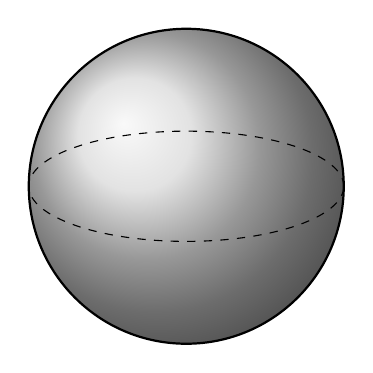
\begin{tikzpicture}[scale=1]
    % Draw the sphere (using ellipse to represent a 3D sphere visually)
    \shade[ball color=gray!30] (0,0) circle (2); % Shaded sphere
    \draw[thick] (0,0) circle (2); % Outline
    \draw[dashed] (0,0) ellipse (2 and 0.7); % Equator line
\end{tikzpicture}
\]

\subsubsection{Cylinder}
\begin{itemize}
    \item A shape with two circular bases and straight sides.
\end{itemize}
\[
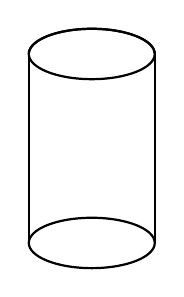
\begin{tikzpicture}[scale=0.8]
    % Draw the bottom ellipse of the cylinder
    \draw[thick] (0,0) ellipse (1 and 0.4); 
    % Draw the top ellipse of the cylinder
    \draw[thick] (0,3) ellipse (1 and 0.4); 
    % Draw the left and right sides of the cylinder
    \draw[thick] (-1,0) -- (-1,3); % Left side
    \draw[thick] (1,0) -- (1,3); % Right side
    % Draw the back and front curves of the top ellipse
    \draw[dashed] (-1,3) arc[start angle=180, end angle=360, x radius=1, y radius=0.4]; % Top back curve
    \draw[thick] (-1,3) arc[start angle=180, end angle=0, x radius=1, y radius=0.4]; % Top front curve
\end{tikzpicture}
\]

\section{Understanding Perimeter and Area}
Perimeter is the distance around the outside of a shape. To find the perimeter, you simply add up the lengths of all the sides of a shape.

\subsection{Example}
To find the perimeter of a rectangle with a length of 5 units and a width of 3 units, add the lengths of all sides:
\[
\text{Perimeter} = 5 + 3 + 5 + 3 = 16 \text{ units}
\]

Area is the amount of space inside a 2D shape. Each shape has its own formula for calculating area.

\subsection{Formulas for Common Shapes}
\subsubsection{Square}
\[
\text{Area} = \text{side} \times \text{side}
\]
For example, if each side of a square is 4 units:
\[
\text{Area} = 4 \times 4 = 16 \text{ square units}
\]

\subsubsection{Rectangle}
\[
\text{Area} = \text{length} \times \text{width}
\]
If a rectangle has a length of 5 units and a width of 3 units:
\[
\text{Area} = 5 \times 3 = 15 \text{ square units}
\]

\subsubsection{Triangle}
\[
\text{Area} = \frac{1}{2} \times \text{base} \times \text{height}
\]
If a triangle has a base of 6 units and a height of 4 units:
\[
\text{Area} = \frac{1}{2} \times 6 \times 4 = 12 \text{ square units}
\]

\subsubsection{Circle}
\[
\text{Area} = \pi \times \text{radius}^2
\]
If a circle has a radius of 3 units:
\[
\text{Area} = 3.14 \times 3^2 = 28.26 \text{ square units} \quad (\text{where } \pi \approx 3.14)
\]

\section{Volume: Measuring 3D Shapes}
Just as we can measure the area of 2D shapes, we can measure the volume of 3D shapes. Volume tells us how much space is inside a 3D object, like how much water a box can hold.

\subsection{Formulas for Common 3D Shapes}
\subsubsection{Cube}
\[
\text{Volume} = \text{side} \times \text{side} \times \text{side}
\]
If each side of the cube is 3 units:
\[
\text{Volume} = 3 \times 3 \times 3 = 27 \text{ cubic units}
\]

\subsubsection{Rectangular Prism}
\[
\text{Volume} = \text{length} \times \text{width} \times \text{height}
\]
If a rectangular prism has dimensions of 4 units (length), 3 units (width), and 5 units (height):
\[
\text{Volume} = 4 \times 3 \times 5 = 60 \text{ cubic units}
\]

\subsubsection{Sphere}
\[
\text{Volume} = \frac{4}{3} \times \pi \times \text{radius}^3
\]
If the radius of the sphere is 2 units:
\[
\text{Volume} \approx \frac{4}{3} \times 3.14 \times 2^3 = 33.51 \text{ cubic units}
\]

\subsubsection{Cylinder}
\[
\text{Volume} = \pi \times \text{radius}^2 \times \text{height}
\]
If a cylinder has a radius of 3 units and a height of 5 units:
\[
\text{Volume} \approx 3.14 \times 3^2 \times 5 = 141.3 \text{ cubic units}
\]

\section{Real-Life Geometry: Applying What We’ve Learned}
Geometry has countless real-world applications. Here are a few examples:

\begin{itemize}
    \item \textbf{Architecture:} When designing a building, architects use geometric shapes to create floor plans, walls, and ceilings. They calculate areas to ensure the building materials fit properly.
    \item \textbf{Gardening:} If you want to fence a rectangular garden, you need to know the perimeter. If you’re planting flowers and want to cover the entire space, you’ll need to calculate the area.
    \item \textbf{Sports:} In sports like basketball, the area of the court determines the playing space, while the volume of the ball affects how it moves through the air.
    \item \textbf{Design:} When creating packaging for a product, designers must consider the volume of the box or container to ensure it holds the right amount of material.
\end{itemize}

\section{Practice Makes Perfect: Let’s Try Some Exercises!}
\subsection{Perimeter and Area}
\begin{itemize}
    \item Find the perimeter of a rectangle with a length of 7 units and a width of 4 units.
    \item Find the area of a triangle with a base of 8 units and a height of 5 units.
    \item Calculate the area of a circle with a radius of 6 units.
\end{itemize}

\subsection{Volume}
\begin{itemize}
    \item Find the volume of a cube with sides of 4 units.
    \item Calculate the volume of a rectangular prism with dimensions 3 units (length), 5 units (width), and 2 units (height).
    \item Find the volume of a cylinder with a radius of 3 units and a height of 7 units.
\end{itemize}

\subsection{Angles}
\begin{itemize}
    \item What type of angle measures 120 degrees?
    \item Measure the angle formed by the hands of a clock at 3:00.
\end{itemize}

\section{Chapter Summary}
\begin{itemize}
    \item Geometry helps us understand the shapes and spaces around us.
    \item We learned about basic 2D and 3D shapes and how to calculate their perimeters, areas, and volumes.
    \item We explored angles and how to measure them.
    \item Geometry is everywhere in our daily lives, from architecture to sports and design.
\end{itemize}

\subsection{Challenge Question}
\begin{enumerate}[label=(\alph*)]
    \item You have a circular garden with a radius of 5 meters. You want to fence the garden and plant flowers in the entire space. How much fencing will you need (circumference), and how many square meters of flowers will you plant (area)?

    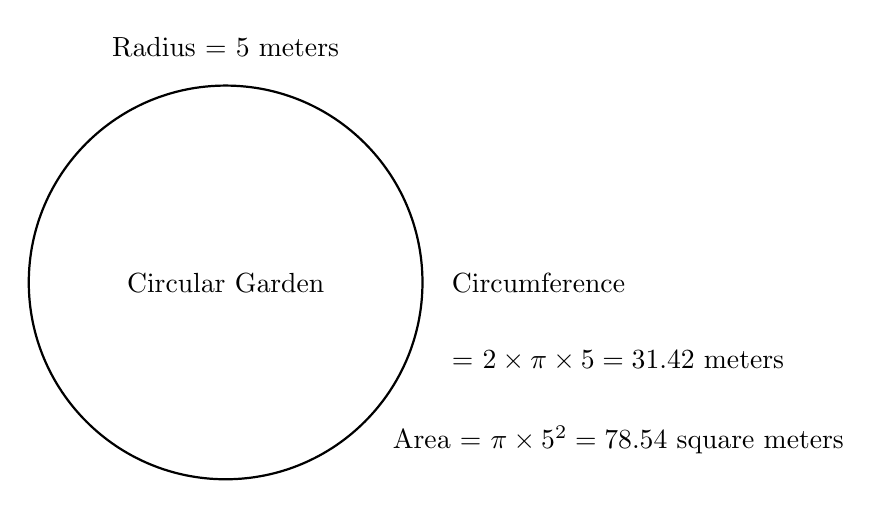
\begin{tikzpicture}
        % Draw the circular garden
        \draw[thick] (0,0) circle(2.5);
        \node[above] at (0,2.75) {Radius = 5 meters};
        \node[right] at (2.75,0) {Circumference};
        \node[right] at (2.75,-1) {= \(2 \times \pi \times 5 = 31.42\) meters};
        \node[right] at (2,-2) {Area = \(\pi \times 5^2 = 78.54\) square meters};
        \node at (0,0) {Circular Garden};
    \end{tikzpicture}

    \item You have a triangular playground with a base of 12 meters and a height of 8 meters. You want to calculate the total area for children to play and determine how much fencing is needed around all three sides if the other two sides are 10 meters and 13 meters. How much fencing will you need (perimeter), and what is the area?

    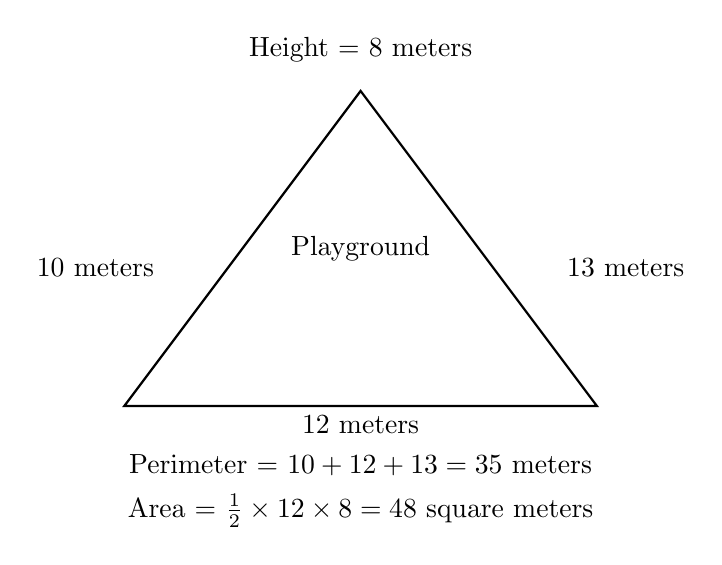
\begin{tikzpicture}
        % Draw the triangular playground
        \draw[thick] (0,0) -- (6,0) -- (3,4) -- cycle;
        \node[below] at (3,0) {12 meters};
        \node[above] at (3,4.25) {Height = 8 meters};
        \node[below left] at (.5,2) {10 meters};
        \node[below right] at (5.5,2) {13 meters};
        \node[below] at (3,-.5) {Perimeter = \(10 + 12 + 13 = 35\) meters};
        \node[below] at (3,-1) {Area = \(\frac{1}{2} \times 12 \times 8 = 48\) square meters};
        \node at (3,2) {Playground};
    \end{tikzpicture}
    \pagebreak
    \item You have a circular swimming pool with a diameter of 10 meters. You want to install a fence around it and calculate the amount of water the pool can hold (area). How much fencing will you need (circumference), and how many square meters of water will the pool hold (area)?
  
    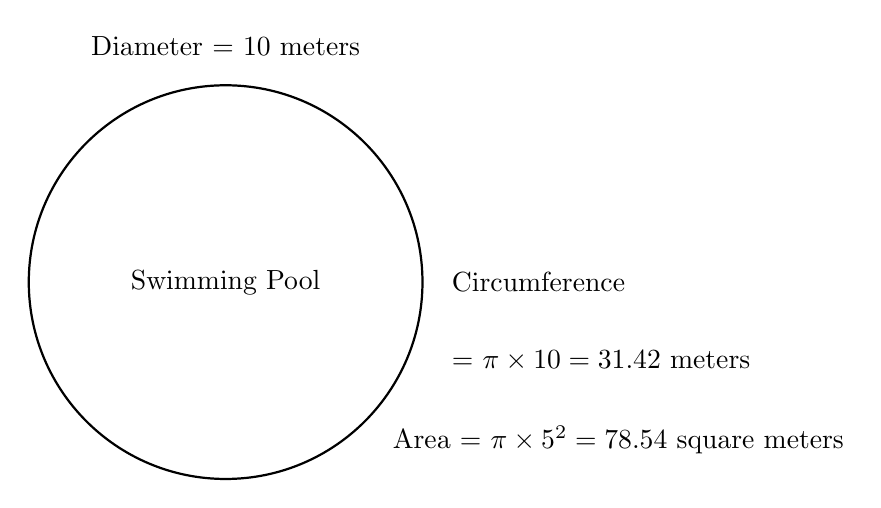
\begin{tikzpicture}
        % Draw the circular swimming pool
        \draw[thick] (0,0) circle(2.5);
        \node[above] at (0,2.75) {Diameter = 10 meters};
        \node[right] at (2.75,0) {Circumference};
        \node[right] at (2.75,-1)  {= \(\pi \times 10 = 31.42\) meters};
        \node[right] at (2,-2) {Area = \(\pi \times 5^2 = 78.54\) square meters};
        \node at (0,0) {Swimming Pool};
    \end{tikzpicture}

    \item You have a trapezoidal parking lot with parallel sides of 20 meters and 10 meters, and the height between the parallel sides is 8 meters. You want to enclose the parking lot with a fence. How much fencing will you need (perimeter), and what is the total area (area)?

    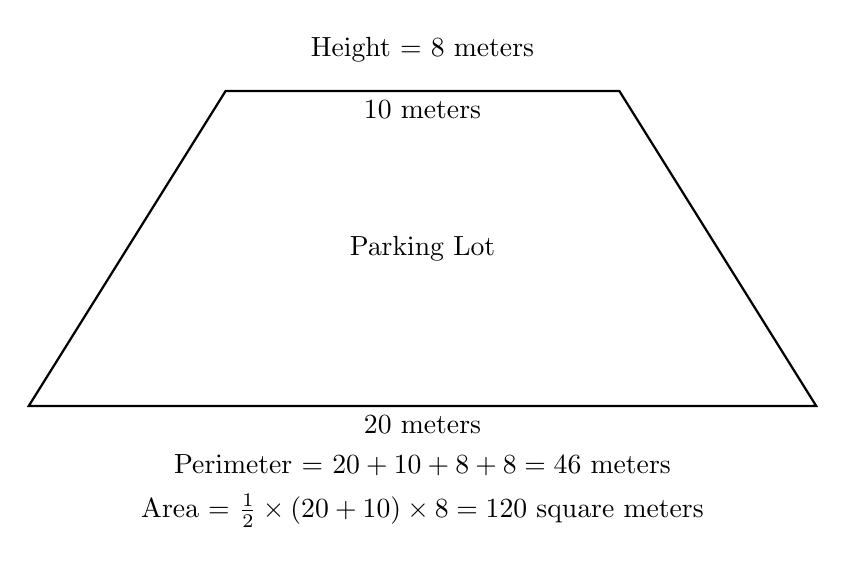
\begin{tikzpicture}
        % Draw the trapezoidal parking lot
        \draw[thick] (0,0) -- (10,0) -- (7.5,4) -- (2.5,4) -- cycle;
        \node[below] at (5,0) {20 meters};
        \node[above] at (5,4.25) {Height = 8 meters};
        \node[below] at (5,4) {10 meters};
        \node[below] at (5,-.5) {Perimeter = \(20 + 10 + 8 + 8 = 46\) meters};
        \node[below] at (5,-1) {Area = \(\frac{1}{2} \times (20 + 10) \times 8 = 120\) square meters};
        \node at (5,2) {Parking Lot};
    \end{tikzpicture}
    \pagebreak
    \item You have a semicircular basketball court with a diameter of 28 meters. You need to install a fence around the curved edge of the court and determine the playing area. How much fencing will you need (perimeter of curved edge), and how many square meters of playing area will you have?

    \begin{tikzpicture}
        % Draw the semicircular basketball court
        \draw[thick] (0,0) arc[start angle=0,end angle=180,radius=7];
        \draw[thick] (0,0) -- (-14,0);
        \node[below] at (-7,-0.5) {Diameter = 28 meters};
        \node[below] at (-7,-1.5) {Curved Perimeter = \(\pi \times 14 = 43.98\) meters};
        \node[below] at (-7,-2.5) {Area = \(\frac{1}{2} \times \pi \times 14^2 = 307.88\) square meters};
        \node at (-7,2) {Basketball Court};
    \end{tikzpicture}
    \pagebreak
    \item You have a pentagonal courtyard where each side is 5 meters long. You plan to fence it and determine the area. How much fencing will you need (perimeter), and what is the area of the courtyard?

    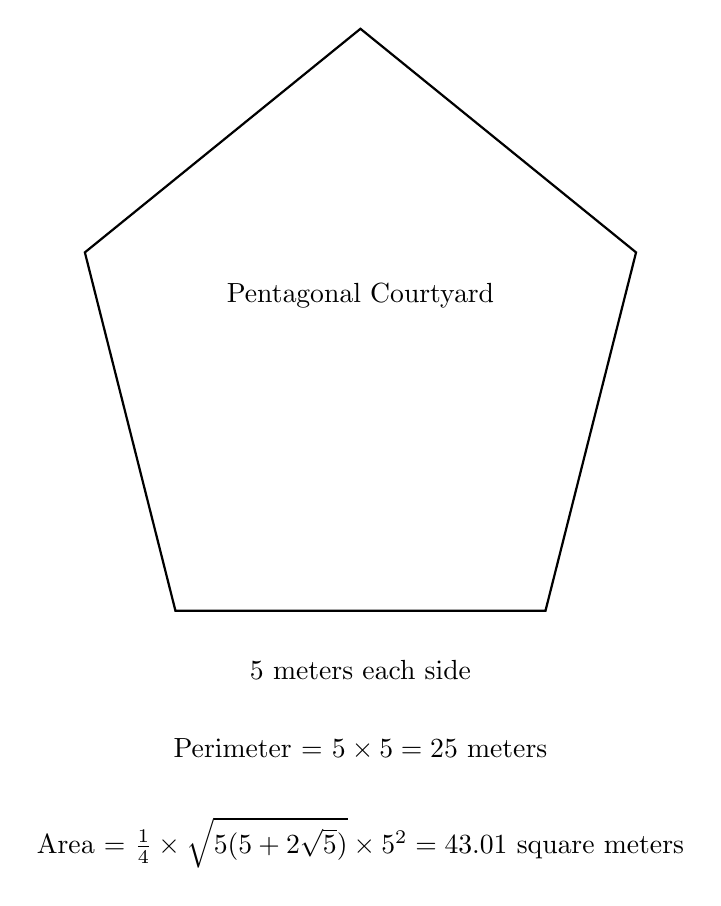
\begin{tikzpicture}
        % Draw the pentagonal courtyard
        \draw[thick] (0,0) -- (4.7,0) -- (5.85,4.55) -- (2.35,7.39) -- (-1.15,4.55) -- cycle;
        \node[below] at (2.35,-0.5) {5 meters each side};
        \node[below] at (2.35,-1.5) {Perimeter = \(5 \times 5 = 25\) meters};
        \node[below] at (2.35,-2.5) {Area = \( \frac{1}{4} \times \sqrt{5(5 + 2\sqrt{5})} \times 5^2 = 43.01\) square meters};
        \node at (2.35,4) {Pentagonal Courtyard};
    \end{tikzpicture}
    \pagebreak
    \item You have an equilateral triangle garden with each side measuring 10 meters. You want to install a fence around it and calculate the planting area. How much fencing will you need (perimeter), and how many square meters of flowers will you plant (area)?

    \begin{tikzpicture}
        % Draw the equilateral triangle garden
        \draw[thick] (0,0) -- (10,0) -- (5,8.66) -- cycle;
        \node[below] at (5,0) {10 meters};
        \node[below] at (5,-1) {Perimeter = \(3 \times 10 = 30\) meters};
        \node[below] at (5,-2) {Area = \(\frac{\sqrt{3}}{4} \times 10^2 = 43.3\) square meters};
        \node at (5,4) {Triangle Garden};
    \end{tikzpicture}

    \item You have an octagonal patio where each side is 4 meters long. You want to install fencing around the entire patio and cover it with tiles. How much fencing will you need (perimeter), and what is the area?

    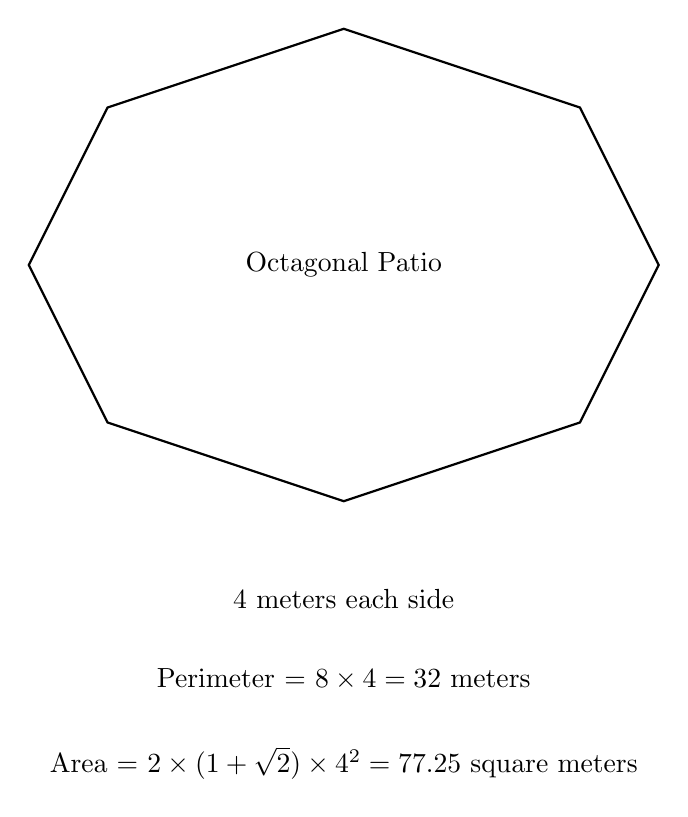
\begin{tikzpicture}
        % Draw the octagonal patio
        \draw[thick] (0,0) -- (3,1) -- (4,3) -- (3,5) -- (0,6) -- (-3,5) -- (-4,3) -- (-3,1) -- cycle;
        \node[below] at (0,-1) {4 meters each side};
        \node[below] at (0,-2) {Perimeter = \(8 \times 4 = 32\) meters};
        \node[below] at (0,-3) {Area = \(2 \times (1 + \sqrt{2}) \times 4^2 = 77.25\) square meters};
        \node at (0,3) {Octagonal Patio};
    \end{tikzpicture}
    \pagebreak
    \item You have a circular classroom rug with a radius of 6 meters. You plan to calculate the length of the border and the total area to be covered by the rug. How much border material will you need (circumference), and how much area will the rug cover?

    \begin{tikzpicture}
        % Draw the circular classroom rug
        \draw[thick] (0,0) circle(6);
        \node[above] at (0,6.5) {Radius = 6 meters};
        \node[below] at (0,-1) {Circumference = \(2 \times \pi \times 6 = 37.70\) meters};
        \node[below] at (0,-2) {Area = \(\pi \times 6^2 = 113.10\) square meters};
        \node at (0,0) {Classroom Rug};
    \end{tikzpicture}
    
\end{enumerate}

\chapter{Data and Probability – Understanding Uncertainty and Making Predictions}

\section{Introduction: Why Data and Probability Matter}
Data is everywhere. Whether it's tracking your daily steps, measuring the weather, or evaluating trends in social media, we rely on data to help us make sense of the world. Data helps us understand patterns, make predictions, and make informed decisions.

Probability, on the other hand, is the branch of math that deals with uncertainty. It helps us understand how likely something is to happen. From deciding whether to bring an umbrella based on the chance of rain, to predicting the outcome of a game, probability plays an essential role in our decision-making process.

In this chapter, we'll dive into the basics of data and probability, exploring how to interpret and use data, and how to calculate the likelihood of different events.

\section{What Is Data?}
Data refers to facts, figures, or information that can be measured and analyzed. Data comes in two main types:

\begin{itemize}
    \item \textbf{Qualitative Data:} Data that describes characteristics or categories. For example, eye color (blue, brown, green) or favorite foods (pizza, pasta, sushi).
    \item \textbf{Quantitative Data:} Data that involves numbers. For example, the number of people in a classroom, the height of a tree, or the temperature outside.
\end{itemize}

We collect and analyze data to uncover patterns, identify trends, and make decisions.

\subsection{Organizing Data}
Data is often organized into tables, graphs, and charts to make it easier to understand.

\textbf{Example:} Imagine you're collecting data on how many books your classmates read in a month. Your data might look like this:

\begin{tabular}{|c|c|}
\hline
Name & Books Read \\
\hline
Sarah & 4 \\
John & 3 \\
Maria & 5 \\
David & 2 \\
\hline
\end{tabular}

From this table, you can easily see how many books each person read and compare the results.

\section{Using Graphs to Represent Data}
Graphs are visual representations of data, making it easier to see patterns and trends. Let’s explore a few common types of graphs:

\subsection{Bar Graph}
Used to compare quantities across different categories. Each bar represents a category, and the height or length of the bar shows the value.

\textbf{Example:} A bar graph showing the number of books read by your classmates:
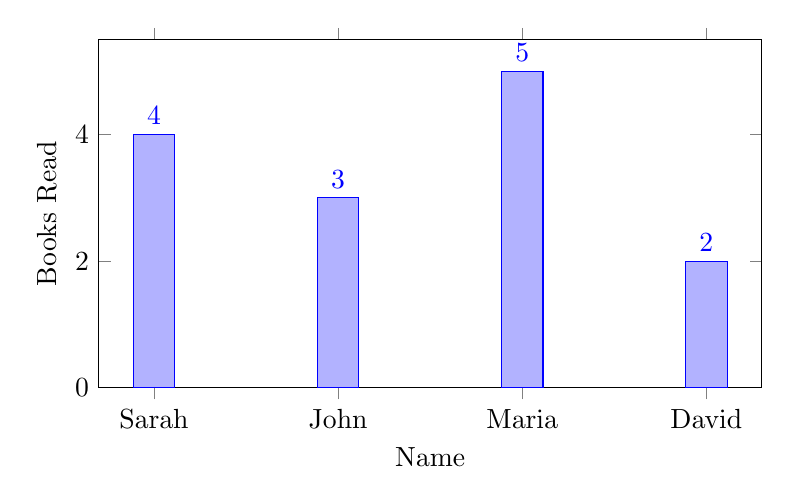
\begin{tikzpicture}
    \begin{axis}[
        ybar,
        symbolic x coords={Sarah, John, Maria, David},
        xtick=data,
        nodes near coords,
        ymin=0,
        ylabel={Books Read},
        xlabel={Name},
        bar width=15pt,
        width=10cm,
        height=6cm
    ]
    \addplot coordinates {(Sarah,4) (John,3) (Maria,5) (David,2)};
    \end{axis}
\end{tikzpicture}
\subsection{Line Graph}
Used to show changes over time. A line connects data points to show how something increases or decreases.

\textbf{Example:} If you track the temperature throughout a month, a line graph could show the daily changes in temperature.
\textbf{Example:} A line graph showing temperature changes over a 30-day period in Fahrenheit:
\begin{center}
    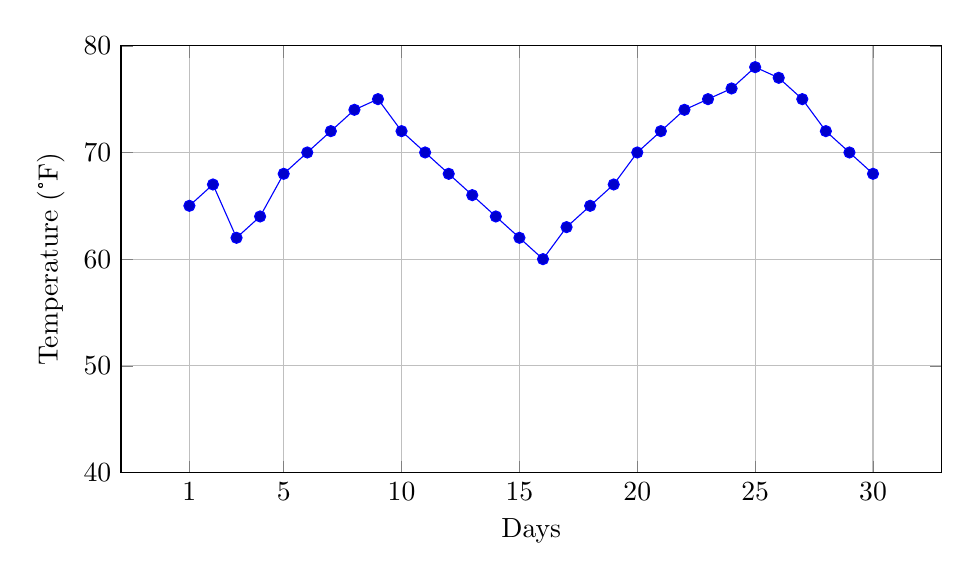
\begin{tikzpicture}
        \begin{axis}[
            xlabel={Days},
            ylabel={Temperature (°F)},
            xtick={1,5,10,15,20,25,30},
            ymin=40,
            ymax=80,
            grid=major,
            width=12cm,
            height=7cm
        ]
        \addplot coordinates {(1,65) (2,67) (3,62) (4,64) (5,68) (6,70) (7,72) 
        (8,74) (9,75) (10,72) (11,70) (12,68) (13,66) (14,64) 
        (15,62) (16,60) (17,63) (18,65) (19,67) (20,70) 
        (21,72) (22,74) (23,75) (24,76) (25,78) (26,77) 
        (27,75) (28,72) (29,70) (30,68)};
        \end{axis}
    \end{tikzpicture}
\end{center}

\subsection{Pie Chart}
Used to show parts of a whole. Each "slice" of the pie represents a percentage of the total.

\textbf{Example:} A pie chart could show the percentage of time you spend on different activities in a day, like studying, exercising, and sleeping.

\begin{center}
    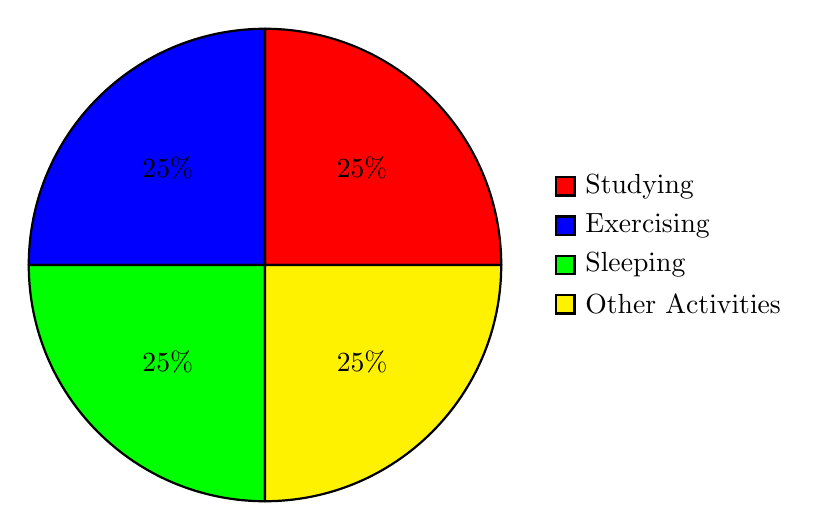
\begin{tikzpicture}
        \pie[
            text=legend,
            radius=3,
            color={red, blue, green, yellow}
        ]{
            25/Studying,
            25/Exercising,
            25/Sleeping,
            25/Other Activities
        }
    \end{tikzpicture}
\end{center}
\section{What Is Probability?}
Probability is the study of how likely something is to happen. It’s a way of measuring uncertainty. The probability of an event can range from 0 to 1:

\begin{itemize}
    \item A probability of 0 means the event is impossible (it will never happen).
    \item A probability of 1 means the event is certain (it will definitely happen).
    \item Any probability between 0 and 1 reflects varying levels of likelihood.
\end{itemize}

\textbf{Example:}

If you're flipping a coin, there are two possible outcomes: heads or tails. Since the coin is fair, each outcome has an equal probability of happening:

\begin{itemize}
    \item The probability of getting heads is $\frac{1}{2}$ or 0.5.
    \item The probability of getting tails is also $\frac{1}{2}$ or 0.5.
\end{itemize}

\section{Calculating Probability}
The basic formula for probability is:

\[
\text{Probability of an event} = \frac{\text{Number of favorable outcomes}}{\text{Total number of possible outcomes}}
\]

\textbf{Example 1: Rolling a Die}

If you roll a standard six-sided die, the probability of rolling a 4 is:

\begin{itemize}
    \item Favorable outcome: 1 (only one side of the die has a 4).
    \item Total possible outcomes: 6 (since the die has six sides).
\end{itemize}

\[
\text{Probability of rolling a 4} = \frac{1}{6}
\]

\textbf{Example 2: Drawing a Card}

If you draw one card from a standard deck of 52 cards, the probability of drawing a heart is:

\begin{itemize}
    \item Favorable outcomes: 13 (since there are 13 hearts in a deck).
    \item Total possible outcomes: 52.
\end{itemize}

\[
\text{Probability of drawing a heart} = \frac{13}{52} = \frac{1}{4}
\]

\section{Complementary and Independent Events}
\subsection{Complementary Events}
Complementary events are two events where one must happen, and the other cannot. For example, when flipping a coin, you either get heads or tails, but not both. The probability of the two events adds up to 1.

If the probability of an event is $P$, then the probability of its complement (the event not happening) is:

\[
\text{Probability of complement} = 1 - P
\]

\textbf{Example:}

If the probability of rain tomorrow is 0.3, the probability that it will not rain is:

\[
1 - 0.3 = 0.7 \text{ or } 70\%
\]

\subsection{Independent Events}
Independent events are events where the outcome of one does not affect the outcome of the other. For example, rolling a die and flipping a coin are independent events because the result of the die does not impact the coin flip.

For independent events, the probability of both events happening is the product of their individual probabilities.

\textbf{Example:}

If the probability of rolling a 6 on a die is $\frac{1}{6}$, and the probability of flipping heads on a coin is $\frac{1}{2}$, the probability of both rolling a 6 and flipping heads is:

\[
\text{Probability of both} = \frac{1}{6} \times \frac{1}{2} = \frac{1}{12}
\]

\section{Making Predictions with Probability}
Probability helps us make predictions about future events based on past data or known probabilities.

\textbf{Example:}

If you know that the chance of rain tomorrow is 60\%, you might decide to bring an umbrella because the probability suggests that it’s more likely to rain than not.

In sports, teams use probability to predict the chances of winning based on previous games, player performance, and conditions like weather or location.

\section{Understanding Averages (Mean, Median, and Mode)}
When analyzing data, it’s often useful to find a measure of central tendency—a number that represents the "middle" or typical value in a set of data. The three most common measures are mean, median, and mode.

\subsection{Mean (Average)}
Add up all the numbers and divide by how many numbers there are.

\textbf{Example:} The mean of 2, 4, 6, and 8 is:

\[
\frac{2 + 4 + 6 + 8}{4} = \frac{20}{4} = 5
\]

\subsection{Median}
The middle number in a sorted list.

\textbf{Example:} The median of 1, 3, and 5 is 3 (because 3 is in the middle).

\subsection{Mode}
The number that appears most often.

\textbf{Example:} In the set 2, 2, 3, 4, 4, 4, the mode is 4 (because it appears three times).

\section{Practice Makes Perfect: Let’s Try Some Exercises!}
\subsection{Probability}
\begin{itemize}
    \item What is the probability of rolling an even number on a six-sided die?
    \item If you flip a coin twice, what is the probability of getting heads both times?
\end{itemize}

\subsection{Data Interpretation}
\begin{itemize}
    \item A class survey found the following number of pets per student: 1, 2, 2, 3, 4, 4, 4, 5. Find the mean, median, and mode of this data.
    \item Draw a bar graph to represent the following data about how many people like different fruits:
    \begin{enumerate}[label=(\alph*)]
        \item Apples: 10
        \item Bananas: 7
         \item Oranges: 5
    \end{enumerate}
\end{itemize}

\section{Real-Life Applications of Data and Probability}
\begin{itemize}
    \item \textbf{Weather Forecasting:} Meteorologists use past data and probability to predict the likelihood of different weather conditions.
    \item \textbf{Health:} Doctors use probability to understand the chances of developing certain conditions based on risk factors like age, genetics, and lifestyle.
    \item \textbf{Games of Chance:} When playing games like dice, cards, or lotteries, probability helps determine the chances of winning.
\end{itemize}

\section{Chapter Summary}
\begin{itemize}
    \item Data helps us collect, organize, and analyze information to understand patterns and make decisions.
    \item Graphs like bar graphs, line graphs, and pie charts help us visualize data.
    \item Probability is the study of uncertainty and helps us measure how likely an event is to happen.
    \item We can calculate the probability of events using the formula: 
    
    \[
    \text{Probability} = \frac{\text{Number of favorable outcomes}}{\text{Total number of possible outcomes}}
    \]
    
    \item Complementary events are those where one event happens, and the other does not, with their probabilities adding up to 1.
    \item Independent events do not affect each other, and the probability of both occurring is the product of their individual probabilities.
    \item Mean, median, and mode are useful measures of central tendency that help summarize data.
\end{itemize}

\subsection{Challenge Questions with Visuals}

\begin{enumerate}
    \item \textbf{Challenge 1: Probability of Rolling a Specific Number}
    \begin{itemize}
        \item What is the probability of rolling a 3 on a six-sided die?
        \item \textbf{Visual:}
        \begin{center}
            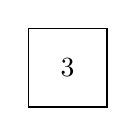
\begin{tikzpicture}
                \draw (0,0) rectangle (1,1);
                \node at (0.5,0.5) {3};
            \end{tikzpicture}
        \end{center}
    \end{itemize}

    \item \textbf{Challenge 2: Probability of Drawing a Specific Card}
    \begin{itemize}
        \item What is the probability of drawing a king from a standard deck of 52 cards?
        \item \textbf{Visual:}
        \begin{center}
            \begin{tikzpicture}
                \node[rectangle, draw, minimum width=1.5cm, minimum height=2cm] at (0,0) {K};
            \end{tikzpicture}
        \end{center}
    \end{itemize}

    \item \textbf{Challenge 3: Probability of Getting Heads Twice}
    \begin{itemize}
        \item If you flip a coin twice, what is the probability of getting heads both times?
        \item \textbf{Visual:}
        \begin{center}
            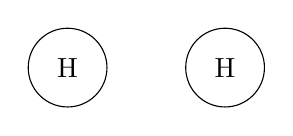
\begin{tikzpicture}
                \node[circle, draw, minimum size=1cm] at (0,0) {H};
                \node[circle, draw, minimum size=1cm] at (2,0) {H};
            \end{tikzpicture}
        \end{center}
    \end{itemize}

    \item \textbf{Challenge 4: Probability of Rolling an Even Number}
    \begin{itemize}
        \item What is the probability of rolling an even number on a six-sided die?
        \item \textbf{Visual:}
        \begin{center}
            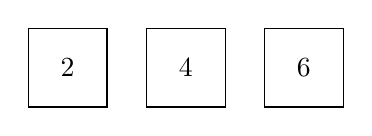
\begin{tikzpicture}
                \draw (0,0) rectangle (1,1);
                \node at (0.5,0.5) {2};
                \draw (1.5,0) rectangle (2.5,1);
                \node at (2,0.5) {4};
                \draw (3,0) rectangle (4,1);
                \node at (3.5,0.5) {6};
            \end{tikzpicture}
        \end{center}
    \end{itemize}

    \item \textbf{Challenge 5: Mean of a Data Set}
    \begin{itemize}
        \item Find the mean of the following data set: 3, 5, 7, 9.
        \item \textbf{Visual:}
        \begin{center}
            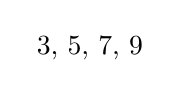
\begin{tikzpicture}
                \node at (0,0) {3, 5, 7, 9};
            \end{tikzpicture}
        \end{center}
    \end{itemize}

    \item \textbf{Challenge 6: Median of a Data Set}
    \begin{itemize}
        \item Find the median of the following data set: 1, 3, 3, 6, 7, 8, 9.
        \item \textbf{Visual:}
        \begin{center}
            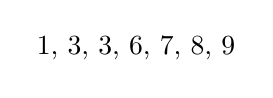
\begin{tikzpicture}
                \node at (0,0) {1, 3, 3, 6, 7, 8, 9};
            \end{tikzpicture}
        \end{center}
    \end{itemize}

    \item \textbf{Challenge 7: Mode of a Data Set}
    \begin{itemize}
        \item Find the mode of the following data set: 4, 4, 5, 5, 5, 6, 7.
        \item \textbf{Visual:}
        \begin{center}
            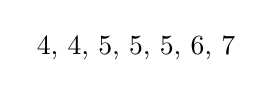
\begin{tikzpicture}
                \node at (0,0) {4, 4, 5, 5, 5, 6, 7};
            \end{tikzpicture}
        \end{center}
    \end{itemize}

    \item \textbf{Challenge 8: Probability of Rolling a Number Greater Than 4}
    \begin{itemize}
        \item What is the probability of rolling a number greater than 4 on a six-sided die?
        \item \textbf{Visual:}
        \begin{center}
            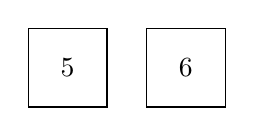
\begin{tikzpicture}
                \draw (0,0) rectangle (1,1);
                \node at (0.5,0.5) {5};
                \draw (1.5,0) rectangle (2.5,1);
                \node at (2,0.5) {6};
            \end{tikzpicture}
        \end{center}
    \end{itemize}

    \item \textbf{Challenge 9: Probability of Drawing an Ace}
    \begin{itemize}
        \item What is the probability of drawing an ace from a standard deck of 52 cards?
        \item \textbf{Visual:}
        \begin{center}
            \begin{tikzpicture}
                \node[rectangle, draw, minimum width=1.5cm, minimum height=2cm] at (0,0) {A};
            \end{tikzpicture}
        \end{center}
    \end{itemize}

    \item \textbf{Challenge 10: Probability of Getting Tails Twice}
    \begin{itemize}
        \item If you flip a coin twice, what is the probability of getting tails both times?
        \item \textbf{Visual:}
        \begin{center}
            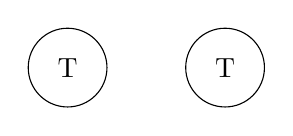
\begin{tikzpicture}
                \node[circle, draw, minimum size=1cm] at (0,0) {T};
                \node[circle, draw, minimum size=1cm] at (2,0) {T};
            \end{tikzpicture}
        \end{center}
    \end{itemize}
    
\end{enumerate}


\chapter{Advanced Algebra – Functions, Graphs, and Equations}

\section{Introduction: The Power of Algebra in Solving Real-World Problems}
Now that you’ve built a strong foundation in basic algebra, we’re ready to explore advanced algebra concepts, such as functions, equations, and graphs. Algebra is about identifying and understanding relationships between numbers, but when those relationships get more complex, we need new tools to make sense of them. That’s where functions and graphs come in.

In this chapter, you’ll learn how to work with different types of equations, understand the concept of functions, and graph relationships between variables. These skills will help you solve more complex problems and visualize how numbers relate to each other.

\section{What Is a Function?}
A function is a rule that assigns exactly one output (result) for each input. You can think of it like a machine: You put in an input (like a number), the function processes it, and you get an output.

Functions are written like this:
\[ f(x) = 2x + 3 \]

In this function:
\begin{itemize}
    \item \( x \) is the input (the number you put in).
    \item \( f(x) \) is the output (what you get after applying the function rule).
    \item The rule is to multiply \( x \) by 2 and then add 3.
\end{itemize}

Example: If \( x = 4 \), then:
\[ f(4) = 2(4) + 3 = 8 + 3 = 11 \]
So, the output is 11 when the input is 4.

Another Example: If \( x = -2 \), then:
\[ f(-2) = 2(-2) + 3 = -4 + 3 = -1 \]

\section{Linear Functions}
A linear function is a type of function where the graph forms a straight line. Linear functions follow the form:
\[ f(x) = mx + b \]

Where:
\begin{itemize}
    \item \( m \) is the slope of the line, representing how steep it is.
    \item \( b \) is the y-intercept, the point where the line crosses the y-axis (when \( x = 0 \)).
\end{itemize}

Example of a Linear Function:
\[ f(x) = 2x + 1 \]
\begin{itemize}
    \item The slope is 2 (for every 1 unit increase in \( x \), \( f(x) \) increases by 2).
    \item The y-intercept is 1 (the line crosses the y-axis at the point (0,1)).
\end{itemize}

Graphing a Linear Function:
\begin{enumerate}
    \item Start by finding the y-intercept (\( b \)).
    \item Use the slope (\( m \)) to plot additional points.
    \item Draw a line through the points.
\end{enumerate}

Example: For \( f(x) = 2x + 1 \):
\begin{itemize}
    \item The y-intercept is 1, so start by plotting the point (0,1).
    \item The slope is 2, meaning for every 1 unit you move to the right, move 2 units up. So plot the point (1,3).
    \item Connect the points with a straight line.
\end{itemize}

\section{Solving Linear Equations}
A linear equation is an equation that makes a straight line when graphed. Solving a linear equation means finding the value of the variable (usually \( x \)) that makes the equation true.

Example: Solve \( 3x + 4 = 13 \).
\begin{enumerate}
    \item Subtract 4 from both sides:
    \[ 3x = 9 \]
    \item Divide both sides by 3:
    \[ x = 3 \]
\end{enumerate}
The solution is \( x = 3 \).

\section{Quadratic Functions}
A quadratic function is more complex than a linear function and has the form:
\[ f(x) = ax^2 + bx + c \]

Where \( a \), \( b \), and \( c \) are constants.

The graph of a quadratic function is a curve called a parabola. Parabolas can open upward or downward, depending on the sign of \( a \):
\begin{itemize}
    \item If \( a > 0 \), the parabola opens upward.
    \item If \( a < 0 \), the parabola opens downward.
\end{itemize}

Example of a Quadratic Function:
\[ f(x) = x^2 - 4x + 3 \]

Graphing a Quadratic Function:
\begin{enumerate}
    \item Find the vertex, which is the highest or lowest point of the parabola.
    \item Plot the vertex and other points on both sides to create a symmetric curve.
\end{enumerate}

\section{Factoring Quadratic Equations}
One method for solving quadratic equations is factoring. This involves rewriting the quadratic equation in a way that allows you to find the values of \( x \) that make the equation true.

Example: Solve \( x^2 - 5x + 6 = 0 \) by factoring.
\begin{enumerate}
    \item Factor the quadratic expression:
    \[ x^2 - 5x + 6 = (x - 2)(x - 3) \]
    \item Set each factor equal to 0:
    \[ x - 2 = 0 \quad \text{or} \quad x - 3 = 0 \]
    \item Solve for \( x \):
    \[ x = 2 \quad \text{or} \quad x = 3 \]
\end{enumerate}
So, the solutions are \( x = 2 \) and \( x = 3 \).

\section{Graphing Quadratic Functions}
Graphing a quadratic function involves finding its key features:
\begin{enumerate}
    \item Vertex: The highest or lowest point of the parabola.
    \item Axis of symmetry: A vertical line that runs through the vertex and divides the parabola into two symmetrical halves.
    \item Intercepts: Points where the graph crosses the x-axis and y-axis.
\end{enumerate}

Example: Graph the quadratic function \( f(x) = x^2 - 4x + 3 \).
\begin{enumerate}
    \item Find the vertex.
    \begin{itemize}
        \item The vertex is at (2, -1).
    \end{itemize}
    \item Find the y-intercept.
    \begin{itemize}
        \item Set \( x = 0 \): \( f(0) = 0^2 - 4(0) + 3 = 3 \).
    \end{itemize}
    \item Plot the points and draw the parabola.
\end{enumerate}

\section{Solving Systems of Linear Equations}
A system of equations is a set of two or more equations that you solve together. A common method is to solve for one variable and substitute it into the other equation.

Example: Solve the system:
\[
\begin{cases}
2x + y = 5 \\
x - y = 1
\end{cases}
\]
\begin{enumerate}
    \item Solve the second equation for \( x \):
    \[ x = y + 1 \]
    \item Substitute \( x = y + 1 \) into the first equation:
    \[ 2(y + 1) + y = 5 \]
    \item Solve for \( y \):
    \[ 2y + 2 + y = 5 \quad \Rightarrow \quad 3y + 2 = 5 \quad \Rightarrow \quad 3y = 3 \quad \Rightarrow \quad y = 1 \]
    \item Substitute \( y = 1 \) back into \( x = y + 1 \):
    \[ x = 1 + 1 = 2 \]
\end{enumerate}
So, the solution is \( x = 2 \) and \( y = 1 \).

\section{Practice Makes Perfect: Let’s Try Some Exercises!}
\subsection*{Functions}
\begin{enumerate}
    \item Evaluate \( f(x) = 3x + 2 \) when \( x = 5 \).
    \item If \( f(x) = 2x^2 - 3x + 1 \), what is \( f(2) \)?
\end{enumerate}

\subsection*{Solving Equations}
\begin{enumerate}
    \item Solve \( 4x - 7 = 9 \).
    \item Solve \( x^2 - 6x + 8 = 0 \) by factoring.
\end{enumerate}

\subsection*{Graphing}
\begin{enumerate}
    \item Graph the linear function \( f(x) = -x + 2 \).
    \item Graph the quadratic function \( f(x) = x^2 + 2x - 3 \).
\end{enumerate}

\section{Real-Life Applications of Functions and Graphs}
\begin{itemize}
    \item \textbf{Business and Economics:} Companies use linear and quadratic equations to model profit and cost functions. By graphing these functions, they can find the optimal production levels to maximize profit.
    \item \textbf{Physics:} Linear and quadratic functions describe the motion of objects, such as the trajectory of a ball when you throw it. Understanding how to graph these functions helps predict where the ball will land.
    \item \textbf{Engineering:} Engineers use functions to model relationships between variables, such as the stress and strain on materials. Graphing these functions helps them design safer structures.
\end{itemize}

\section{Chapter Summary}
\begin{itemize}
    \item A function is a rule that assigns one output for each input. Linear functions form straight lines, while quadratic functions form parabolas.
    \item The equation of a linear function is \( f(x) = mx + b \), where \( m \) is the slope and \( b \) is the y-intercept.
    \item Quadratic functions take the form \( f(x) = ax^2 + bx + c \) and can be graphed as parabolas.
    \item You can solve linear equations by isolating the variable, and solve quadratic equations by factoring or graphing.
    \item Systems of equations involve solving two or more equations together to find where their graphs intersect.
\end{itemize}

\section*{Challenge Question}
Graph the function \( f(x) = 2x^2 - 4x + 1 \), find the vertex, and identify where the graph crosses the x-axis and y-axis.
\chapter{Understanding Change Over Time – Change and Motion}

\section{Introduction}
Calculus is the branch of mathematics that focuses on change. While algebra helps us solve for unknown values and geometry deals with shapes and spaces, calculus answers questions about how things change over time, how fast things move, or how quantities accumulate.

Don’t let the idea of calculus intimidate you! At its core, calculus is simply a way of understanding rates of change and accumulation. Whether it’s predicting the speed of a car, calculating areas under curves, or modeling population growth, calculus provides the tools to solve these kinds of problems.

In this chapter, we’ll explore the basics of derivatives and integrals, the two main concepts of calculus, and how they help us describe change and motion.

\section{What Is a Derivative?}
A derivative tells us how a function is changing at any given point. It measures the rate of change or the slope of a curve at a specific point. In simpler terms, it answers questions like:
\begin{itemize}
    \item How fast is a car moving at a specific moment?
    \item How quickly is the population growing?
\end{itemize}

\textbf{Notation:} the following is a table of calculus notations for derivatives and integrals.

\begin{table}[h!]
    \centering
    \begin{tabular}{|l|p{3cm}|p{5cm}|}
        \hline
        \textbf{Notation} & \textbf{Definition} & \textbf{Description} \\
        \hline
        $f'(x)$ & First Derivative of $f(x)$ & Represents the rate of change or slope of $f(x)$ at a point. \\
        \hline
        $\frac{dy}{dx}$ & Derivative of $y$ with respect to $x$ & Common notation for the derivative when $y = f(x)$. \\
        \hline
        $\frac{d}{dx}\left[ f(x) \right]$ & Derivative Operator & Used to denote taking the derivative of $f(x)$ with respect to $x$. \\
        \hline
        $f''(x)$ & Second Derivative of $f(x)$ & Represents the rate of change of $f'(x)$; indicates concavity. \\
        \hline
        $\frac{d^2y}{dx^2}$ & Second Derivative of $y$ with respect to $x$ & Measures how the rate of change itself is changing. \\
        \hline
        $\int f(x) \, dx$ & Indefinite Integral of $f(x)$ & The antiderivative of $f(x)$, representing the area under the curve of $f(x)$. \\
        \hline
        $\int_a^b f(x) \, dx$ & Definite Integral from $a$ to $b$ & Represents the exact area under $f(x)$ from $x = a$ to $x = b$. \\
        \hline
        $\lim_{h \to 0} \frac{f(x+h) - f(x)}{h}$ & Limit Definition of Derivative & Defines the derivative as the limit of the average rate of change. \\
        \hline
        $\partial y / \partial x$ & Partial Derivative of $y$ with respect to $x$ & Used for functions with multiple variables, finding the derivative with respect to one variable while holding others constant. \\
        \hline
    \end{tabular}
    \caption{Common Calculus Notations for Derivatives and Integrals}
\end{table}


\subsection{The Concept of Slope}
In algebra, the slope of a line is a measure of its steepness, and it tells us how fast one variable changes with respect to another. In calculus, the slope is used to describe the instantaneous rate of change of a function.

\subsection{Example}

For a linear function like \( f(x) = 2x + 3 \), the slope is constant. The derivative of this function is 2, meaning the rate of change is the same no matter where you are on the line.

\begin{center}
    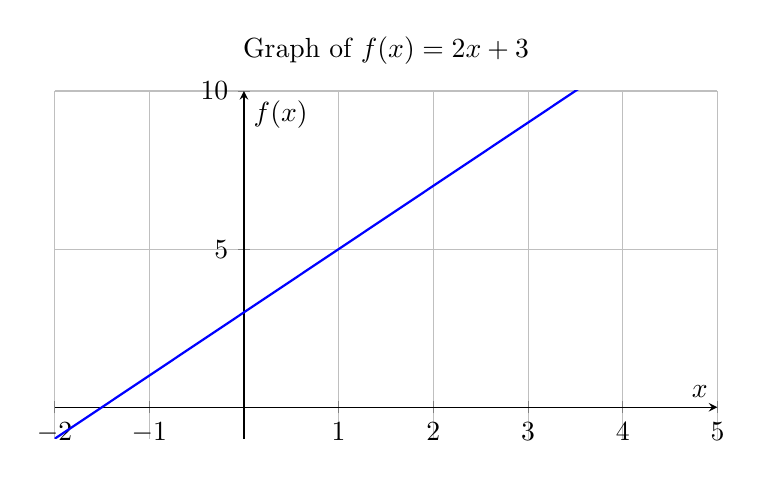
\begin{tikzpicture}
        \begin{axis}[
            axis lines = middle,
            xlabel = \(x\),
            ylabel = {\(f(x)\)},
            ymin=-1, ymax=10,
            xmin=-2, xmax=5,
            grid = major,
            width=10cm,
            height=6cm,
            domain=-2:5,
            samples=100,
            title={Graph of \( f(x) = 2x + 3 \)}
        ]
        \addplot[blue, thick] {2*x + 3};
    \end{axis}
    \end{tikzpicture}
    \captionof{figure}{Graph of the linear function \( f(x) = 2x + 3 \). The slope is constant across the entire line.}
\end{center}

But what happens when the function isn’t a straight line? For functions that curve, like \( f(x) = x^2 \), the slope (or rate of change) varies depending on the point. The derivative helps us figure out the slope at any point along the curve.

\begin{center}
    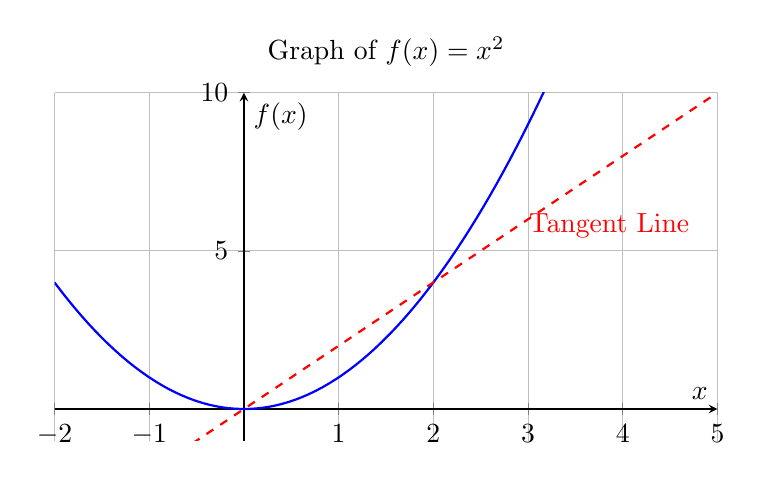
\begin{tikzpicture}
        \begin{axis}[
            axis lines = middle,
            xlabel = \(x\),
            ylabel = {\(f(x)\)},
            ymin=-1, ymax=10,
            xmin=-2, xmax=5,
            grid = major,
            width=10cm,
            height=6cm,
            domain=-2:5,
            samples=100,
            title={Graph of \( f(x) = x^2 \)}
        ]
        \addplot[blue, thick] {x^2};
        \addplot[red, dashed, thick, domain=-2:5] {2*x} node [pos=0.7, right] {Tangent Line};
    \end{axis}
    \end{tikzpicture}
    \captionof{figure}{Graph of the quadratic function \( f(x) = x^2 \). The red dashed line shows a tangent at a point, illustrating the slope at that specific point. The slope of the tangent line represents the derivative of the function at that point, which gives the instantaneous rate of change of the function. As the point moves along the curve, the slope of the tangent line changes, reflecting the varying rate of change of the function. This demonstrates how the derivative provides valuable information about the behavior of the function at different points.}
\end{center}

\section{Finding Derivatives}

The derivative of a function helps us find the rate of change, which can be calculated using specific rules. These rules make it easier to determine how different functions change.

\begin{itemize}
    \item \textbf{Power Rule:} If $f(x) = x^n$, then the derivative is $f'(x) = n \cdot x^{n-1}$.
    
    \begin{center}
        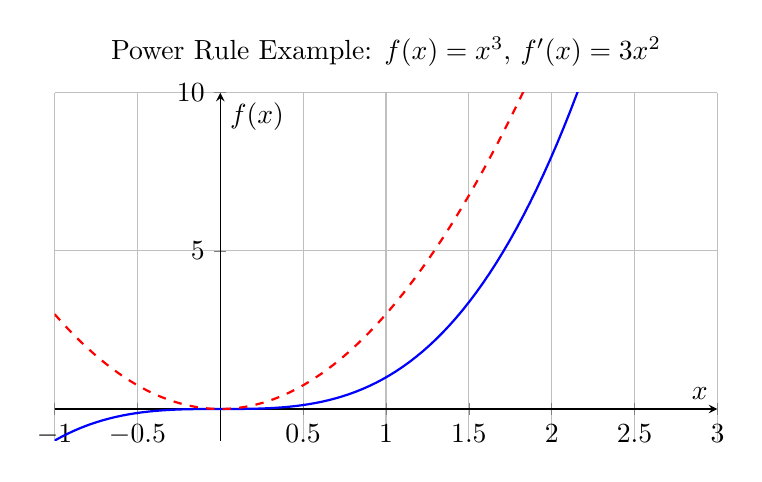
\begin{tikzpicture}
            \begin{axis}[
                axis lines = middle,
                xlabel = $x$,
                ylabel = {$f(x)$},
                ymin=-1, ymax=10,
                xmin=-1, xmax=3,
                grid = major,
                width=10cm,
                height=6cm,
                domain=-1:3,
                samples=100,
                title={Power Rule Example: $f(x) = x^3$, $f'(x) = 3x^2$}
            ]
            \addplot[blue, thick] {x^3};
            \addplot[red, dashed, thick] {3*x^2};
        \end{axis}
        \end{tikzpicture}
        \captionof{figure}{Graph of $f(x) = x^3$ (blue) and its derivative $f'(x) = 3x^2$ (red dashed). The derivative represents the rate of change of the curve.}
    \end{center}

    \item \textbf{Constant Rule:} The derivative of a constant function is zero.
    
    \begin{center}
        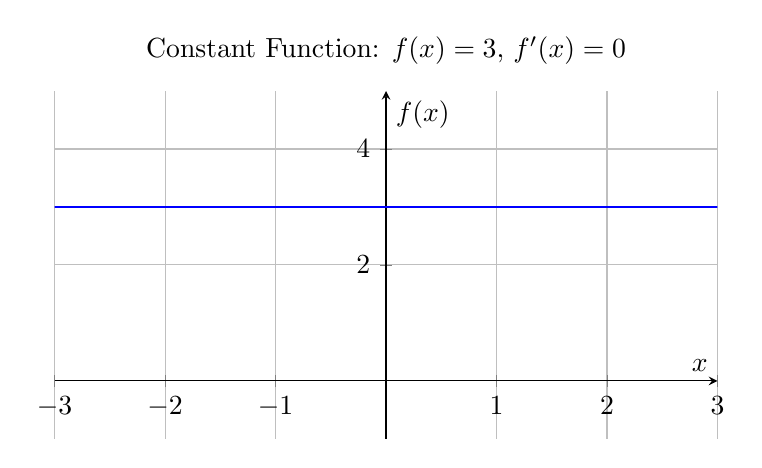
\begin{tikzpicture}
            \begin{axis}[
                axis lines = middle,
                xlabel = $x$,
                ylabel = {$f(x)$},
                ymin=-1, ymax=5,
                xmin=-3, xmax=3,
                grid = major,
                width=10cm,
                height=6cm,
                title={Constant Function: $f(x) = 3$, $f'(x) = 0$}
            ]
            \addplot[blue, thick] {3};
        \end{axis}
        \end{tikzpicture}
        \captionof{figure}{Graph of the constant function $f(x) = 3$. The slope of this function is zero everywhere, hence $f'(x) = 0$.}
    \end{center}

    \item \textbf{Sum Rule:} The derivative of the sum of functions is the sum of their derivatives.
    
    \begin{center}
        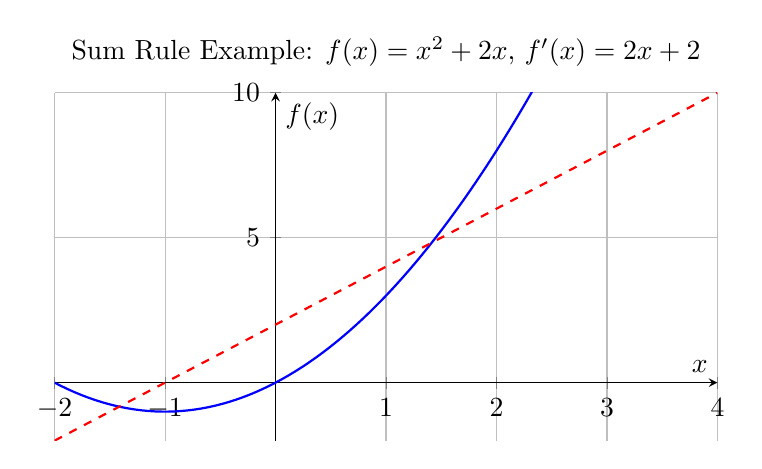
\begin{tikzpicture}
            \begin{axis}[
                axis lines = middle,
                xlabel = $x$,
                ylabel = {$f(x)$},
                ymin=-2, ymax=10,
                xmin=-2, xmax=4,
                grid = major,
                width=10cm,
                height=6cm,
                domain=-2:4,
                samples=100,
                title={Sum Rule Example: $f(x) = x^2 + 2x$, $f'(x) = 2x + 2$}
            ]
            \addplot[blue, thick] {x^2 + 2*x};
            \addplot[red, dashed, thick] {2*x + 2};
        \end{axis}
        \end{tikzpicture}
        \captionof{figure}{Graph of $f(x) = x^2 + 2x$ (blue) and its derivative $f'(x) = 2x + 2$ (red dashed). The derivative is the sum of the derivatives of $x^2$ and $2x$.}
    \end{center}

    \item \textbf{Product Rule:} The derivative of the product of two differentiable functions is given by:
    
    \[ f(x) = g(x) \cdot h(x) \quad \Rightarrow \quad f'(x) = g'(x) \cdot h(x) + g(x) \cdot h'(x) \]
    
    \textbf{Example:} If $f(x) = x^2 \cdot \sin(x)$:
    \begin{enumerate}
        \item Set $g(x) = x^2$ and $h(x) = \sin(x)$.
        \item Compute $g'(x) = 2x$ and $h'(x) = \cos(x)$.
        \item Substitute into the Product Rule:
        \[ f'(x) = (2x) \cdot \sin(x) + x^2 \cdot \cos(x) \]
    \end{enumerate}
    
    \begin{center}
        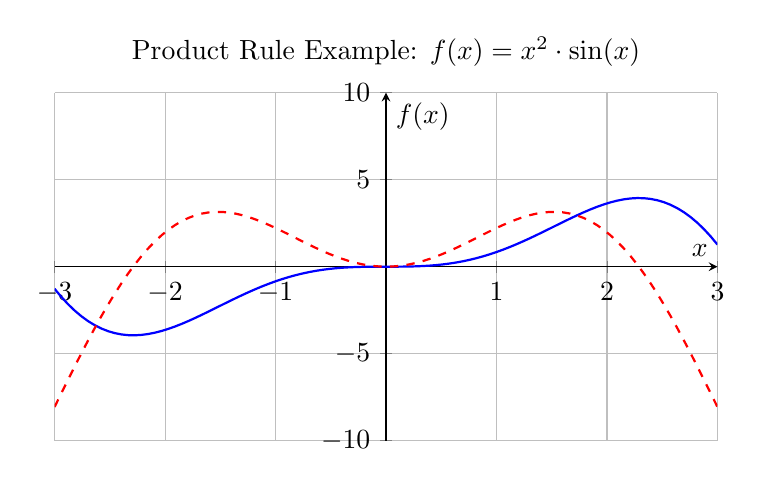
\begin{tikzpicture}
            \begin{axis}[
                axis lines = middle,
                xlabel = $x$,
                ylabel = {$f(x)$},
                ymin=-10, ymax=10,
                xmin=-3, xmax=3,
                grid = major,
                width=10cm,
                height=6cm,
                domain=-3:3,
                samples=100,
                title={Product Rule Example: $f(x) = x^2 \cdot \sin(x)$}
            ]
            \addplot[blue, thick] {x^2 * sin(deg(x))};
            \addplot[red, dashed, thick] {2*x*sin(deg(x)) + x^2*cos(deg(x))};
        \end{axis}
        \end{tikzpicture}
        \captionof{figure}{Graph of $f(x) = x^2 \cdot \sin(x)$ (blue) and its derivative $f'(x)$ (red dashed).}
    \end{center}

    \begin{center}
        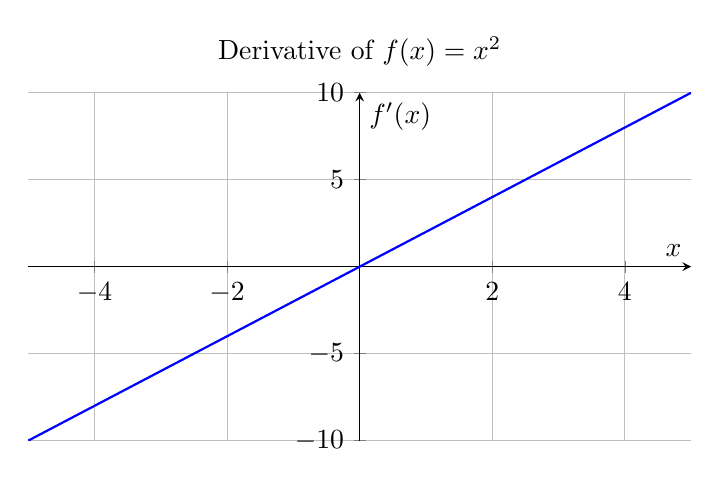
\begin{tikzpicture}
            \begin{axis}[
                axis lines = middle,
                xlabel = $x$,
                ylabel = {$f'(x)$},
                ymin=-10, ymax=10,
                xmin=-5, xmax=5,
                grid = major,
                width=10cm,
                height=6cm,
                domain=-5:5,
                samples=100,
                title={Derivative of $f(x) = x^2$}
                ]
            \addplot[blue, thick] {2*x};
            \end{axis}
        \end{tikzpicture}
        \captionof{figure}{Graph of the derivative $f'(x) = 2x$ of the function $f(x) = x^2$. The slope of $f(x)$ changes depending on the value of $x$.}
    \end{center}
\end{itemize}


\subsection{Basic Rules for Derivatives}
\begin{enumerate}
    \item \textbf{Power Rule:} For any function of the form $f(x) = x^n$, where $n$ is a constant, the derivative is:
    \[ f'(x) = n \cdot x^{n-1} \]
    \textbf{Examples:}
    \begin{itemize}
        \item For $f(x) = x^2$, the derivative is: $f'(x) = 2x$
        \item For $f(x) = x^3$, the derivative is: $f'(x) = 3x^2$
    \end{itemize}
    
    \item \textbf{Constant Rule:} The derivative of a constant is always 0. This is because a constant does not change, so its rate of change is 0.
    \textbf{Example:}
    \begin{itemize}
        \item For $f(x) = 7$, the derivative is $f'(x) = 0$.
    \end{itemize}
    
    \item \textbf{Sum and Difference Rule:} If you have two functions being added or subtracted, you can find the derivative of each part separately.
    \textbf{Example:}
    \begin{itemize}
        \item For $f(x) = 3x^2 + 4x$, the derivative is: $f'(x) = 6x + 4$
    \end{itemize}
\end{enumerate}

\subsection{Interpreting Derivatives}
The derivative gives you the slope of a curve at any point. If the slope is positive, the function is increasing at that point; if the slope is negative, the function is decreasing.

\section{Applications of Derivatives}
Derivatives are incredibly useful in real-world scenarios. Let’s look at a few practical examples:
\begin{enumerate}
    \item \textbf{Velocity:} If you know the position of an object as a function of time, the derivative of that function gives you the object’s velocity, or the rate of change of position.

    \textbf{Example:} Suppose the position of a car over time is given by \( f(t) = t^2 \).
    \begin{itemize}
        \item The derivative, \( f'(t) = 2t \), tells us the car’s velocity at any time \( t \).
    \end{itemize}
    
    \begin{center}
        \begin{tikzpicture}
            \begin{axis}[
                axis lines = middle,
                xlabel = $t$,
                ylabel = {$f(t)$},
                ymin=-1, ymax=10,
                xmin=-1, xmax=4,
                grid = major,
                width=10cm,
                height=6cm,
                domain=0:4,
                samples=100,
                title={Position and Velocity: $f(t) = t^2$, $f'(t) = 2t$}
            ]
            \addplot[blue, thick] {x^2};
            \addplot[red, dashed, thick] {2*x};
            \legend{$f(t) = t^2$, $f'(t) = 2t$}
        \end{axis}
        \end{tikzpicture}
        \captionof{figure}{Graph of position \( f(t) = t^2 \) (blue) and its velocity \( f'(t) = 2t \) (red dashed). The slope of the position function represents the car's velocity over time.}
    \end{center}

    \item \textbf{Optimization:} Businesses use derivatives to find maximum profits or minimum costs. By taking the derivative of a profit or cost function, companies can determine when profits are at their highest or when costs are at their lowest.

    \textbf{Example:} Suppose the profit function of a business is \( P(x) = -2x^2 + 12x + 5 \), where \( x \) is the number of items produced and sold.
    \begin{itemize}
        \item To maximize profit, we find the critical points by setting the derivative to zero:
        \[ P'(x) = -4x + 12 \]
        \[ -4x + 12 = 0 \Rightarrow x = 3 \]
        \item At \( x = 3 \), the business achieves maximum profit.
    \end{itemize}

    \begin{center}
        \begin{tikzpicture}
            \begin{axis}[
                axis lines = middle,
                xlabel = $x$,
                ylabel = {$P(x)$},
                ymin=-10, ymax=20,
                xmin=0, xmax=6,
                grid = major,
                width=10cm,
                height=6cm,
                domain=0:6,
                samples=100,
                title={Profit Function: $P(x) = -2x^2 + 12x + 5$}
            ]
            \addplot[blue, thick] {-2*x^2 + 12*x + 5};
            \addplot[red, mark=*] coordinates {(3,23)};
            \node at (axis cs:3,23) [above right] {$\text{Max Profit at } x=3$};
        \end{axis}
        \end{tikzpicture}
        \captionof{figure}{Graph of the profit function \( P(x) = -2x^2 + 12x + 5 \) with a maximum at \( x = 3 \).}
    \end{center}

    \item \textbf{Tangent Lines:} The derivative of a function at a point gives the slope of the tangent line to the curve at that point. A tangent line is a straight line that touches the curve at exactly one point and represents the best linear approximation of the curve near that point.

    \textbf{Example:} Let \( f(x) = x^2 \). To find the tangent line at \( x = 1 \):
    \begin{itemize}
        \item Compute the derivative: \( f'(x) = 2x \).
        \item At \( x = 1 \), the slope of the tangent line is \( f'(1) = 2 \).
        \item The equation of the tangent line at \( x = 1 \) is given by:
        \[ y = f(1) + f'(1)(x - 1) = 1 + 2(x - 1) = 2x - 1 \]
    \end{itemize}

    \begin{center}
        \begin{tikzpicture}
            \begin{axis}[
                axis lines = middle,
                xlabel = $x$,
                ylabel = {$f(x)$},
                ymin=-1, ymax=5,
                xmin=-1, xmax=3,
                grid = major,
                width=10cm,
                height=6cm,
                domain=-1:3,
                samples=100,
                title={Tangent Line at $x = 1$ for $f(x) = x^2$}
            ]
            \addplot[blue, thick] {x^2};
            \addplot[red, dashed, thick] {2*x - 1};
            \legend{$f(x) = x^2$, $y = 2x - 1$}
        \end{axis}
        \end{tikzpicture}
        \captionof{figure}{Graph of \( f(x) = x^2 \) (blue) and its tangent line at \( x = 1 \), \( y = 2x - 1 \) (red dashed). The tangent line touches the curve at exactly one point, providing a linear approximation.}
    \end{center}
\end{enumerate}


\section{What Is an Integral?}
While derivatives focus on how things change, integrals help us calculate how much has accumulated over time. An integral measures the area under a curve.

Imagine you’re tracking the speed of a car over time. The integral of the speed function gives you the total distance the car has traveled.

\subsection{The Concept of Area}
In algebra, you can find the area of simple shapes like rectangles and triangles. In calculus, integrals allow you to find the area under curves, even if the shape is irregular.

\section{Finding Integrals}
Just like derivatives, there are rules for finding integrals. These rules help you calculate the total accumulation or area under a curve.

\subsection{Basic Rules for Integrals}
\begin{enumerate}
    \item \textbf{Power Rule for Integrals:} For any function of the form \( f(x) = x^n \), the integral is:
    \[
    \int x^n \, dx = \frac{x^{n+1}}{n+1} + C
    \]
    Where \( C \) is a constant (because integrals can have multiple solutions based on starting points).
    \textbf{Example:}
    \begin{itemize}
        \item For \( f(x) = x^2 \), the integral is: \( \int x^2 \, dx = \frac{x^3}{3} + C \)
    \end{itemize}
    \item \textbf{Constant Rule for Integrals:} The integral of a constant is the constant times \( x \).
    \textbf{Example:}
    \begin{itemize}
        \item For \( f(x) = 5 \), the integral is: \( \int 5 \, dx = 5x + C \)
    \end{itemize}
    \item \textbf{Sum and Difference Rule for Integrals:} You can integrate each part of a sum or difference separately.
    \textbf{Example:}
    \begin{itemize}
        \item For \( f(x) = 3x^2 + 2x \), the integral is: \( \int (3x^2 + 2x) \, dx = x^3 + x^2 + C \)
    \end{itemize}
\end{enumerate}

\section{Applications of Integrals}
Integrals have many practical applications, especially when you need to calculate totals, such as:
\begin{enumerate}
    \item \textbf{Area Under a Curve:} If you want to calculate the total area under a curve (for example, finding the total distance a car has traveled), integrals provide the solution.
    \textbf{Example:}
    \begin{itemize}
        \item If the velocity of a car is given by \( f(t) = 2t \), the integral of this function gives the distance traveled: \( \int 2t \, dt = t^2 + C \)
    \end{itemize}
    \item \textbf{Accumulating Quantities:} If you know how something is changing, you can use integrals to find the total amount accumulated over time. For example, if you know the rate at which water is flowing into a tank, you can use an integral to find the total amount of water in the tank after a certain time.
    \item \textbf{Economics and Finance:} Integrals are used in economics to calculate things like consumer surplus and producer surplus by finding the area under demand or supply curves.
\end{enumerate}

\section{Fundamental Theorem of Calculus}
The Fundamental Theorem of Calculus links derivatives and integrals. It states that:
\begin{enumerate}
    \item The derivative of the integral of a function is the function itself.
    \item The integral of the derivative of a function gives you the accumulated value of the function.
\end{enumerate}
In simple terms, derivatives and integrals are two sides of the same coin—one describes how something is changing, while the other describes how much has accumulated.

\section{Practice Makes Perfect: Let’s Try Some Exercises!}
\subsection{Derivatives}
\begin{enumerate}
    \item Find the derivative of \( f(x) = 4x^3 \).
    \item Find the derivative of \( f(x) = x^2 + 3x + 2 \).
\end{enumerate}

\subsection{Integrals}
\begin{enumerate}
    \item Find the integral of \( f(x) = x^2 \).
    \item Find the integral of \( f(x) = 3x + 5 \).
\end{enumerate}

\subsection{Applications}
\begin{enumerate}
    \item A car’s position is given by \( f(t) = t^2 + 2t \). Find the car’s velocity by taking the derivative.
    \item Find the area under the curve \( f(x) = 2x \) between \( x = 0 \) and \( x = 3 \).
\end{enumerate}

\section{Real-Life Applications of Calculus}
\begin{itemize}
    \item \textbf{Physics:} Calculus helps in understanding motion, forces, and energy. Derivatives are used to find velocities and accelerations, while integrals calculate distances and areas under curves.
    \item \textbf{Engineering:} Engineers use calculus to model systems that involve changes, such as heat flow, structural loads, and electrical circuits.
    \item \textbf{Medicine:} In pharmacokinetics, integrals help calculate the total amount of a drug in the bloodstream over time, while derivatives describe how quickly the drug is absorbed or eliminated.
\end{itemize}

\section{Chapter Summary}
\begin{itemize}
    \item Derivatives measure the rate of change of a function. They tell us how fast something is changing at a particular moment.
    \item Integrals measure accumulation. They help us calculate the total amount of something, such as the area under a curve.
    \item The Fundamental Theorem of Calculus connects derivatives and integrals, showing that they are inverse operations.
    \item Calculus has many real-world applications, from physics and engineering to economics and medicine.
\end{itemize}

\section{Challenge Question}
A car’s velocity is given by \( v(t) = 3t^2 \), where \( t \) is time in seconds. Find the car’s total distance traveled between \( t = 0 \) and \( t = 4 \) seconds by using an integral.
\chapter{Trigonometry – Angles and Waves}

\section{Introduction: Understanding the World Through Trigonometry}
Trigonometry is the study of the relationships between the angles and sides of triangles, but it goes far beyond geometry. It has applications in fields like physics, engineering, architecture, and even sound and light waves. Whenever you hear terms like "sine" or "cosine," you're dealing with trigonometry.
In this chapter, we’ll explore the basics of trigonometry, focusing on how to understand angles, work with trigonometric functions, and apply these concepts to solve real-world problems involving triangles and waves.

\section{Right Triangles and Trigonometric Ratios}
The most common triangle in trigonometry is the right triangle, which has one angle equal to 90 degrees. The relationship between the sides and angles of a right triangle forms the foundation of trigonometry.
In any right triangle, we have three sides:
\begin{itemize}
    \item \textbf{Hypotenuse:} The longest side, opposite the right angle.
    \item \textbf{Opposite side:} The side opposite the angle you’re focusing on.
    \item \textbf{Adjacent side:} The side next to the angle you’re focusing on (but not the hypotenuse).
\end{itemize}

\begin{center}
\begin{tikzpicture}
    % Draw the triangle
    \draw[thick] (0,0) -- (4,0) -- (4,3) -- cycle;

    % Labels for sides
    \node at (2, -0.3) {Adjacent};
    \node at (5,1) {Opposite};
    \node at (1.5, 2) {Hypotenuse};

    % 90 degree angle square
    \draw (3.7,0) rectangle +(0.3,0.3);
    \node at (4.5, 0.2) {$90^\circ$};

    % Angle label
    \node at (0.5, 0.2) {$\theta$};

    % Arrowed lines for sides
    \draw[thick, <->] (4,0) -- (4,3); % Opposite
    \draw[thick, <->] (0,0) -- (4,0); % Adjacent
    \draw[thick, <->] (0,0) -- (4,3); % Hypotenuse

\end{tikzpicture}
\end{center}

\subsection{Trigonometric Ratios}
The three basic trigonometric functions are sine (sin), cosine (cos), and tangent (tan). These functions relate the angles of a triangle to the lengths of its sides.
For any angle $\theta$ in a right triangle:
\begin{enumerate}
    \item \textbf{Sine (sin):}
    \[
    \sin(\theta) = \frac{\text{opposite}}{\text{hypotenuse}}
    \]
    \item \textbf{Cosine (cos):}
    \[
    \cos(\theta) = \frac{\text{adjacent}}{\text{hypotenuse}}
    \]
    \item \textbf{Tangent (tan):}
    \[
    \tan(\theta) = \frac{\text{opposite}}{\text{adjacent}}
    \]
\end{enumerate}
These ratios allow us to calculate missing side lengths or angles in right triangles.

\section{Using Trigonometric Ratios}
Let’s look at an example of how to use these trigonometric functions to solve problems involving right triangles.

\subsection{Example 1: Finding the Length of a Side}
In a right triangle, if the angle $\theta = 30^\circ$ and the hypotenuse is 10 units long, how long is the opposite side?
\begin{enumerate}
    \item Use the sine function:
    \[
    \sin(30^\circ) = \frac{\text{opposite}}{10}
    \]
    \item Look up or recall that $\sin(30^\circ) = 0.5$:
    \[
    0.5 = \frac{\text{opposite}}{10}
    \]
    \item Solve for the opposite side:
    \[
    \text{opposite} = 0.5 \times 10 = 5 \text{ units}
    \]
\end{enumerate}

\section{The Pythagorean Theorem}
The Pythagorean Theorem is another essential tool for working with right triangles. It relates the lengths of the sides of a right triangle:
\[
a^2 + b^2 = c^2
\]
Where:
\begin{itemize}
    \item $a$ and $b$ are the lengths of the legs (the two shorter sides),
    \item $c$ is the length of the hypotenuse.
\end{itemize}

\subsection{Example}
If one leg of a right triangle is 3 units long and the other leg is 4 units long, what is the length of the hypotenuse?
\begin{enumerate}
    \item Plug the values into the Pythagorean Theorem:
    \[
    3^2 + 4^2 = c^2
    \]
    \item Simplify:
    \[
    9 + 16 = c^2 \quad \Rightarrow \quad 25 = c^2
    \]
    \item Solve for $c$:
    \[
    c = \sqrt{25} = 5 \text{ units}
    \]
    The hypotenuse is 5 units long.
\end{enumerate}

\section{Angles in Degrees and Radians}
In trigonometry, angles can be measured in two different units:
\begin{enumerate}
    \item \textbf{Degrees:} The most familiar way to measure angles (e.g., $90^\circ$, $180^\circ$).
    \item \textbf{Radians:} A more mathematical way to measure angles, often used in calculus and advanced math. One full revolution around a circle is $2\pi$ radians, which is equivalent to $360^\circ$.
\end{enumerate}

\subsection{Converting Between Degrees and Radians}
To convert from degrees to radians, use the formula:
\[
\text{radians} = \frac{\pi}{180^\circ} \times \text{degrees}
\]

\subsubsection{Example}
Convert $90^\circ$ to radians:
\[
90^\circ = \frac{\pi}{180^\circ} \times 90^\circ = \frac{\pi}{2} \text{ radians}
\]

To convert from radians to degrees, use the formula:
\[
\text{degrees} = \frac{180^\circ}{\pi} \times \text{radians}
\]

\subsubsection{Example}
Convert $\frac{\pi}{4}$ radians to degrees:
\[
\frac{\pi}{4} \text{ radians} = \frac{180^\circ}{\pi} \times \frac{\pi}{4} = 45^\circ
\]

\section{The Unit Circle}
The unit circle is a circle with a radius of 1, centered at the origin of a coordinate plane. It’s a fundamental tool in trigonometry because it allows us to define the trigonometric functions for all angles, not just those in right triangles.
In the unit circle:
\begin{itemize}
    \item The x-coordinate of a point on the circle represents $\cos(\theta)$.
    \item The y-coordinate represents $\sin(\theta)$.
\end{itemize}

\subsection{Key Angles on the Unit Circle}
\begin{itemize}
    \item $\sin(0^\circ) = 0$ and $\cos(0^\circ) = 1$
    \item $\sin(90^\circ) = 1$ and $\cos(90^\circ) = 0$
    \item $\sin(180^\circ) = 0$ and $\cos(180^\circ) = -1$
    \item $\sin(270^\circ) = -1$ and $\cos(270^\circ) = 0$
\end{itemize}
Knowing these values allows you to solve trigonometric problems for many different angles.

\section{Graphs of Sine and Cosine}
The sine and cosine functions can be graphed as waves. These functions are periodic, meaning they repeat at regular intervals.

\subsection{Graph of Sine (sin)}
The sine wave starts at 0, rises to 1, falls back to 0, drops to -1, and returns to 0. This pattern repeats every $360^\circ$ or $2\pi$ radians.

\subsection{Graph of Cosine (cos)}
The cosine wave starts at 1, drops to 0, falls to -1, rises back to 0, and returns to 1. Like the sine wave, it repeats every $360^\circ$ or $2\pi$ radians.

\section{Applications of Trigonometry}
Trigonometry is incredibly useful in many real-world situations. Here are a few examples:
\begin{enumerate}
    \item \textbf{Engineering and Architecture:} Trigonometry helps engineers and architects design buildings, bridges, and other structures. They use trigonometric functions to calculate forces, angles, and distances.
    \item \textbf{Physics:} Trigonometry is used in physics to describe the motion of objects, especially those that move in waves, like sound and light. It’s also used to model oscillations, such as the swinging of a pendulum.
    \item \textbf{Navigation:} Trigonometry helps pilots and sailors navigate by using angles and distances on maps. It’s also crucial for understanding how GPS systems work.
    \item \textbf{Music and Sound Waves:} The sine and cosine functions describe sound waves. The pitch of a musical note is related to the frequency of the wave, which can be modeled using trigonometry.
\end{enumerate}

\section{Practice Makes Perfect: Let’s Try Some Exercises!}
\subsection{Trigonometric Ratios}
\begin{enumerate}
    \item Find $\sin(45^\circ)$ if the hypotenuse is 10 units.
    \item Find $\cos(30^\circ)$ if the hypotenuse is 8 units.
\end{enumerate}

\subsection{Right Triangles}
\begin{enumerate}
    \item Use the Pythagorean Theorem to find the missing side of a right triangle with legs of length 5 and 12.
    \item Find the tangent of an angle $\theta$ in a right triangle where the opposite side is 4 units and the adjacent side is 3 units.
\end{enumerate}

\subsection{Graphing}
\begin{enumerate}
    \item Sketch the graph of $y = \sin(x)$ for $0^\circ \leq x \leq 360^\circ$.
    \item Sketch the graph of $y = \cos(x)$ for $0^\circ \leq x \leq 360^\circ$.
\end{enumerate}

\section{Real-Life Applications of Trigonometry}
\begin{itemize}
    \item \textbf{Surveying:} Trigonometry is used in surveying to measure distances and angles between points on land.
    \item \textbf{Astronomy:} Astronomers use trigonometry to calculate the distances between stars and planets. The orbits of planets can be described using trigonometric functions.
    \item \textbf{Medical Imaging:} In technologies like MRI and ultrasound, trigonometry helps to create images of the inside of the human body by analyzing waves.
\end{itemize}

\section{Chapter Summary}
\begin{itemize}
    \item Sine (sin), cosine (cos), and tangent (tan) are the fundamental trigonometric ratios that describe the relationship between the sides and angles of a right triangle.
    \item The Pythagorean Theorem helps us find missing side lengths in right triangles.
    \item Angles can be measured in degrees or radians, and the unit circle is a key tool for understanding trigonometric functions for all angles.
    \item Sine and cosine functions can be graphed as periodic waves, repeating at regular intervals.
    \item Trigonometry has many practical applications, from engineering and architecture to physics, navigation, and music.
\end{itemize}

\section{Challenge Questions}

\begin{enumerate}

    % Question 1
    \item Find the height of a tree given the angle of elevation from a point 30 meters away is $45^\circ$.
    \\ 
    \textbf{Visual:} A right triangle showing the tree as the vertical side, the distance to the tree as the base, and an angle of elevation of $45^\circ$.

    % Question 2
    \item A ladder leans against a wall at an angle of $60^\circ$ with the ground. If the ladder is 10 meters long, how far is the base of the ladder from the wall?
    \\ 
    \textbf{Visual:} A ladder forming a right triangle with the wall and the ground, showing the $60^\circ$ angle and a hypotenuse of 10 meters.

    % Question 3
    \item Given a triangle with sides $a = 8$, $b = 15$, and an included angle $\theta = 60^\circ$, find the length of the third side.
    \\ 
    \textbf{Visual:} A non-right triangle showing two known sides and the included $60^\circ$ angle, where you need to find the third side.

    % Question 4
    \item The sine of angle $\alpha$ in a right triangle is $\frac{3}{5}$. What is the cosine of the complementary angle $\beta$?
    \\ 
    \textbf{Visual:} A right triangle labeled with $\alpha$ and $\beta$, indicating their complementarity.

    % Question 5
    \item A point $P$ on the unit circle corresponds to an angle of $120^\circ$. Find the coordinates of point $P$.
    \\ 
    \textbf{Visual:} A unit circle showing the angle $120^\circ$ and point $P$ on the circumference.

    % Question 6
    \item Find the length of the shadow cast by a 5-meter pole when the sun's angle of elevation is $30^\circ$.
    \\ 
    \textbf{Visual:} A right triangle formed by the pole, its shadow, and the angle of elevation of $30^\circ$.

    % Question 7
    \item Solve for $x$ in the equation $\tan(x) = \frac{1}{\sqrt{3}}$ for $0^\circ \leq x < 360^\circ$.
    \\ 
    \textbf{Visual:} A unit circle with the tangent line indicating points that have a tangent value of $\frac{1}{\sqrt{3}}$.

    % Question 8
    \item If $\sin(\theta) = 0.6$, find $\cos(\theta)$ using the Pythagorean identity.
    \\ 
    \textbf{Visual:} A right triangle with $\sin(\theta) = 0.6$, illustrating the relationship between the opposite side and hypotenuse.

    % Question 9
    \item Find the area of a triangle with sides $a = 7$, $b = 9$, and angle $C = 45^\circ$ between them.
    \\ 
    \textbf{Visual:} A non-right triangle with two sides labeled $a$ and $b$, and angle $C = 45^\circ$ marked.

    % Question 10
    \item A ferris wheel has a radius of 20 meters. If a rider is at an angle of $\frac{\pi}{3}$ radians from the horizontal, what is their height above the ground if the wheel's center is 25 meters above the ground?
    \\ 
    \textbf{Visual:} A ferris wheel diagram with a rider at angle $\frac{\pi}{3}$ and a radius of 20 meters, indicating the height from the ground.

\end{enumerate}


\chapter{Abstract Math – Logic, Sets, and Proofs}

\section{Introduction: The Structure Behind Mathematics}
At the heart of mathematics lies a set of fundamental ideas: logic, sets, and proofs. These concepts form the foundation for nearly everything we’ve learned so far. In this chapter, we’ll take a closer look at the building blocks of mathematical reasoning and the tools mathematicians use to demonstrate whether something is true or false.

Logic, sets, and proofs may seem abstract at first, but they are powerful tools for solving problems and understanding the structure of mathematics itself. Whether you're proving a theorem, analyzing data, or coding a computer algorithm, these ideas are key to thinking clearly and solving problems systematically.

\section{What Is Logic?}
Logic is the study of reasoning. In math, logic helps us determine whether statements are true or false and how to combine these statements to make new conclusions.

\subsection{Logical Statements}
A statement in logic is a sentence that is either true or false. For example:
\begin{itemize}
    \item "2 + 2 = 4" is a true statement.
    \item "5 is greater than 10" is a false statement.
\end{itemize}
We often use symbols to represent logical statements:
\begin{itemize}
    \item \( p \) might represent "2 + 2 = 4."
    \item \( q \) might represent "5 is greater than 10."
\end{itemize}

\subsection{Logical Operations}
We can combine logical statements using logical operations, such as:
\begin{enumerate}
    \item \textbf{AND ( \(\land\) )}: Both statements must be true for the combined statement to be true.
    \begin{itemize}
        \item For example, \( p \land q \) means "p AND q."
        \item If \( p \) is true and \( q \) is false, \( p \land q \) is false.
    \end{itemize}
    \item \textbf{OR ( \(\lor\) )}: If at least one of the statements is true, the combined statement is true.
    \begin{itemize}
        \item \( p \lor q \) means "p OR q."
        \item If \( p \) is true and \( q \) is false, \( p \lor q \) is still true.
    \end{itemize}
    \item \textbf{NOT ( \(\neg\) )}: This operation negates a statement. If a statement is true, its negation is false, and vice versa.
    \begin{itemize}
        \item \( \neg p \) means "NOT p."
        \item If \( p \) is true, \( \neg p \) is false.
    \end{itemize}
\end{enumerate}

\subsection{Example}
\begin{itemize}
    \item Let \( p \) represent "It is raining."
    \item Let \( q \) represent "I have an umbrella."
\end{itemize}
If it is raining (\( p \) is true) and I have an umbrella (\( q \) is true), the statement \( p \land q \) (It is raining AND I have an umbrella) is true.

If it is not raining (\( p \) is false), the statement \( p \land q \) is false, even if I still have an umbrella.

\section{What Is a Set?}
A set is a collection of distinct objects or elements. These objects can be anything: numbers, letters, or even other sets.

\subsection{Notation}
We use curly brackets to represent a set. For example:
\begin{itemize}
    \item \( A = \{1, 2, 3, 4\} \) represents a set of four numbers.
    \item \( B = \{a, b, c\} \) represents a set of three letters.
\end{itemize}

\subsection{Elements of a Set}
The objects within a set are called elements. We use the symbol \( \in \) to indicate that something is an element of a set. For example:
\begin{itemize}
    \item \( 3 \in A \) means "3 is an element of set \( A \)."
    \item \( d \notin B \) means "d is not an element of set \( B \)."
\end{itemize}

\subsection{Types of Sets}
\begin{enumerate}
    \item \textbf{Finite Set}: A set with a limited number of elements.
    \begin{itemize}
        \item \( A = \{1, 2, 3\} \) is a finite set.
    \end{itemize}
    \item \textbf{Infinite Set}: A set with an unlimited number of elements.
    \begin{itemize}
        \item The set of all natural numbers \( \{1, 2, 3, 4, \dots\} \) is infinite.
    \end{itemize}
    \item \textbf{Empty Set}: A set with no elements, denoted by \( \emptyset \) or \( \{\} \).
\end{enumerate}

\section{Set Operations}
Just as we can perform operations on numbers, we can perform operations on sets. The most common set operations are union, intersection, and difference.

\subsection{Union ( \(\cup\) )}
The union of two sets combines all the elements from both sets. If an element is in either set (or both), it’s in the union.

Example: If \( A = \{1, 2, 3\} \) and \( B = \{3, 4, 5\} \), the union of \( A \) and \( B \) is:
\[ A \cup B = \{1, 2, 3, 4, 5\} \]

\subsection{Intersection ( \(\cap\) )}
The intersection of two sets contains only the elements that are in both sets.

Example: If \( A = \{1, 2, 3\} \) and \( B = \{3, 4, 5\} \), the intersection of \( A \) and \( B \) is:
\[ A \cap B = \{3\} \]

\subsection{Difference ( - )}
The difference between two sets contains the elements in one set but not the other.

Example: If \( A = \{1, 2, 3\} \) and \( B = \{3, 4, 5\} \), the difference of \( A \) and \( B \) (elements in \( A \) but not in \( B \)) is:
\[ A - B = \{1, 2\} \]

\section{What Is a Proof?}
A proof is a logical argument that demonstrates the truth of a mathematical statement. Proofs are the backbone of mathematics, ensuring that our conclusions are reliable and based on solid reasoning.

\subsection{Types of Proofs}
\begin{enumerate}
    \item \textbf{Direct Proof}: You start with known facts and use logical steps to arrive at the conclusion.
    \begin{itemize}
        \item Example: Prove that if \( n \) is an even number, then \( n^2 \) is even.
        \begin{itemize}
            \item Proof: If \( n \) is even, we can write \( n = 2k \) for some integer \( k \).
            \item \( n^2 = (2k)^2 = 4k^2 = 2(2k^2) \), which is clearly divisible by 2, so \( n^2 \) is even.
        \end{itemize}
    \end{itemize}
    \item \textbf{Proof by Contradiction}: You assume the opposite of what you're trying to prove, show that this leads to a contradiction, and conclude that the original statement must be true.
    \begin{itemize}
        \item Example: Prove that there is no largest prime number.
        \begin{itemize}
            \item Proof: Assume there is a largest prime number, \( p \). Now consider the number \( N = p_1 \times p_2 \times \dots \times p_n + 1 \), where \( p_1, p_2, \dots, p_n \) are all prime numbers up to \( p \).
            \item \( N \) is not divisible by any of these primes, which contradicts the assumption that \( p \) is the largest prime. Therefore, there is no largest prime number.
        \end{itemize}
    \end{itemize}
    \item \textbf{Proof by Induction}: This method is used to prove statements that hold for an infinite number of cases (often for natural numbers). It involves two steps:
    \begin{itemize}
        \item \textbf{Base Case}: Prove that the statement is true for the first value (often \( n = 1 \)).
        \item \textbf{Inductive Step}: Assume the statement is true for some \( n = k \) and then prove it is true for \( n = k + 1 \).
        \item Example: Prove that the sum of the first \( n \) natural numbers is \( \frac{n(n+1)}{2} \).
        \begin{itemize}
            \item Base Case: For \( n = 1 \), the sum is 1, which matches \( \frac{1(1+1)}{2} = 1 \).
            \item Inductive Step: Assume the formula holds for \( n = k \), meaning: \( 1 + 2 + \dots + k = \frac{k(k+1)}{2} \). Now prove it for \( n = k + 1 \):
            \[ 1 + 2 + \dots + k + (k+1) = \frac{k(k+1)}{2} + (k+1) = \frac{(k+1)(k+2)}{2} \]
            Therefore, the statement holds for \( n = k + 1 \), completing the proof by induction.
        \end{itemize}
    \end{itemize}
\end{enumerate}

\section{Mathematical Logic and Proofs in Real Life}
Logic and proofs might seem theoretical, but they have many real-world applications:
\begin{enumerate}
    \item \textbf{Computer Science}: Logic is the foundation of programming. Algorithms, conditional statements, and decision-making all rely on logical operations and reasoning.
    \item \textbf{Cryptography}: The security of modern cryptographic systems (used to protect online data) is based on proofs of mathematical statements about prime numbers and number theory.
    \item \textbf{Legal and Scientific Arguments}: Logic helps construct valid arguments, whether you're writing a legal brief or conducting a scientific experiment. Proofs and logical reasoning ensure that conclusions are reliable and based on evidence.
\end{enumerate}

\section{Practice Makes Perfect: Let’s Try Some Exercises!}
\subsection{Logic}
\begin{enumerate}
    \item Let \( p \) represent "It is sunny" and \( q \) represent "I will go for a walk." Write the following in logical notation:
    \begin{itemize}
        \item "It is not sunny, and I will go for a walk."
        \item "If it is sunny, then I will go for a walk."
    \end{itemize}
\end{enumerate}

\subsection{Sets}
\begin{enumerate}
    \item If \( A = \{1, 2, 3\} \) and \( B = \{3, 4, 5\} \), find \( A \cup B \), \( A \cap B \), and \( A - B \).
    \item If \( C = \{a, b, c\} \) and \( D = \{c, d, e\} \), find \( C \cup D \) and \( C \cap D \).
\end{enumerate}

\subsection{Proofs}
\begin{enumerate}
    \item Prove that the sum of two even numbers is always even.
    \item Use proof by contradiction to show that \( \sqrt{2} \) is irrational.
\end{enumerate}

\section{Chapter Summary}
\begin{itemize}
    \item Logic is the study of reasoning, and it helps us determine whether statements are true or false.
    \item Sets are collections of objects, and we can perform operations like union, intersection, and difference on sets.
    \item Proofs are logical arguments that demonstrate the truth of mathematical statements. They come in many forms, such as direct proofs, proof by contradiction, and proof by induction.
    \item Logic, sets, and proofs are fundamental to mathematics and have many practical applications, from computer science to cryptography.
\end{itemize}

\section*{Challenge Question}
Prove that the product of any two odd numbers is always odd. Use a direct proof to show your result.

\chapter{Understanding Infinity – Limits and Advanced Topics}

\section{Introduction: Exploring the Concept of Infinity}
The idea of infinity is one of the most profound and mind-expanding concepts in mathematics. Unlike a regular number, infinity represents something that never ends or something that is larger than any number you can imagine. While infinity seems abstract, it is a central idea in many advanced math topics, from calculus to set theory and beyond.

In this chapter, we will explore the concept of limits, which help us understand how numbers behave as they approach infinity (or other values). We will also explore other fascinating advanced topics related to infinity, such as infinite sequences, series, and the nature of different "sizes" of infinity.

\section{What Is a Limit?}
In mathematics, a limit describes the value that a function or sequence "approaches" as the input (or index) gets closer to a certain point or as it heads toward infinity.

\subsection{Understanding Limits}
A limit helps us answer questions like:
\begin{itemize}
    \item "What happens to a function as $x$ gets larger and larger?"
    \item "What value does a function approach as $x$ gets closer to a particular number?"
\end{itemize}

\textbf{Example:} Consider the function $f(x) = \frac{1}{x}$. As $x$ gets larger and larger, the value of $f(x)$ gets closer to 0. We say:
\[
\lim_{x \to \infty} \frac{1}{x} = 0
\]
This means that as $x$ approaches infinity, the value of $f(x)$ approaches 0, but it never actually reaches 0.

\subsection{Left-Hand and Right-Hand Limits}
Sometimes, we’re interested in how a function behaves as it approaches a specific value from the left or the right.
\begin{itemize}
    \item The left-hand limit looks at how the function behaves as the input approaches from values smaller than the target value.
    \item The right-hand limit looks at how the function behaves as the input approaches from values larger than the target value.
\end{itemize}

\textbf{Example:} For the function $f(x) = \frac{1}{x-1}$, we might ask what happens as $x$ approaches 1 from both sides:
\[
\lim_{x \to 1^-} \frac{1}{x-1} = -\infty \quad \text{and} \quad \lim_{x \to 1^+} \frac{1}{x-1} = \infty
\]
This means that as $x$ approaches 1 from the left, $f(x)$ goes to negative infinity, and as $x$ approaches from the right, $f(x)$ goes to positive infinity.

\section{Understanding Infinite Sequences}
An infinite sequence is an ordered list of numbers that continues forever. Each number in the sequence is called a term, and the position of the term in the sequence is called its index.

\textbf{Example of an Infinite Sequence:}
Consider the sequence:
\[
1, \frac{1}{2}, \frac{1}{3}, \frac{1}{4}, \dots
\]
This sequence continues indefinitely, and the general term for the sequence is $\frac{1}{n}$, where $n$ is the index of the term.

As $n$ gets larger, the terms in the sequence get smaller, and we can use limits to describe this behavior:
\[
\lim_{n \to \infty} \frac{1}{n} = 0
\]
This means that as $n$ approaches infinity, the terms in the sequence approach 0.

\subsection{Converging vs. Diverging Sequences}
\begin{itemize}
    \item A sequence converges if the terms get closer and closer to a particular value.
    \item A sequence diverges if the terms do not approach a specific value and instead grow without bound or oscillate.
\end{itemize}

\textbf{Example:}
\begin{itemize}
    \item The sequence $\frac{1}{n}$ converges to 0 as $n \to \infty$.
    \item The sequence $n^2$ diverges because the terms grow larger and larger without bound as $n \to \infty$.
\end{itemize}

\section{What Is an Infinite Series?}
An infinite series is the sum of the terms of an infinite sequence. Just as with sequences, some series converge (add up to a finite value), while others diverge (grow without bound).

\textbf{Example of an Infinite Series:}
Consider the series:
\[
S = 1 + \frac{1}{2} + \frac{1}{4} + \frac{1}{8} + \dots
\]
This is called a geometric series because each term is a fixed fraction of the previous term. In this case, each term is half of the previous one.

We can find the sum of this geometric series by using the formula:
\[
S = \frac{a}{1 - r}
\]
Where:
\begin{itemize}
    \item $a$ is the first term,
    \item $r$ is the common ratio between terms (in this case, $r = \frac{1}{2}$).
\end{itemize}

For the series above:
\[
S = \frac{1}{1 - \frac{1}{2}} = \frac{1}{\frac{1}{2}} = 2
\]
So, the sum of this infinite series is 2, meaning the series converges.

\subsection{Diverging Series}
Not all infinite series converge. For example, the series:
\[
1 + 1 + 1 + 1 + \dots
\]
clearly grows without bound, so it diverges.

\section{Understanding Asymptotes}
An asymptote is a line that a graph approaches but never touches. Asymptotes often appear in graphs of functions that involve infinity, helping us understand the behavior of a function as it gets closer to certain points or heads toward infinity.

\subsection{Vertical Asymptote}
A vertical asymptote occurs when a function increases or decreases without bound as it approaches a specific $x$-value.

\textbf{Example:} The function $f(x) = \frac{1}{x-2}$ has a vertical asymptote at $x = 2$, because the function approaches infinity as $x$ gets closer to 2 from the right, and negative infinity as $x$ approaches from the left.

\subsection{Horizontal Asymptote}
A horizontal asymptote describes the behavior of a function as $x$ heads toward infinity. It represents a value that the function gets closer to but never actually reaches.

\textbf{Example:} For $f(x) = \frac{1}{x}$, the horizontal asymptote is $y = 0$, because as $x \to \infty$, the function approaches 0.

\section{Different Sizes of Infinity}
One of the most surprising facts about infinity is that not all infinities are the same size! This concept was first explored by the mathematician Georg Cantor, who showed that some infinite sets are "larger" than others.

\subsection{Countable vs. Uncountable Infinity}
\begin{itemize}
    \item A set is countably infinite if its elements can be put in one-to-one correspondence with the natural numbers. For example, the set of all whole numbers $\{0, 1, 2, 3, \dots\}$ is countably infinite.
    \item A set is uncountably infinite if it cannot be listed in this way. For example, the set of all real numbers between 0 and 1 is uncountably infinite, meaning that this set is "larger" than the set of natural numbers.
\end{itemize}

Cantor’s work showed that even within infinity, there are different levels of "size," revolutionizing our understanding of math.

\section{Practice Makes Perfect: Let’s Try Some Exercises!}
\subsection{Limits}
\begin{enumerate}
    \item Find $\lim_{x \to \infty} \frac{1}{x+3}$.
    \item Evaluate $\lim_{x \to 2} \frac{1}{x-2}$.
\end{enumerate}

\subsection{Sequences}
\begin{enumerate}
    \item Determine whether the sequence $\frac{1}{n^2}$ converges or diverges as $n \to \infty$.
    \item Find the limit of the sequence $2^n$ as $n \to \infty$.
\end{enumerate}

\subsection{Series}
\begin{enumerate}
    \item Determine if the series $1 + \frac{1}{2} + \frac{1}{3} + \dots$ converges or diverges.
    \item Find the sum of the geometric series $2 + 1 + \frac{1}{2} + \frac{1}{4} + \dots$.
\end{enumerate}

\section{Real-Life Applications of Infinity and Limits}
\begin{itemize}
    \item \textbf{Physics:} Limits and infinity are crucial in physics, especially in understanding concepts like velocity, acceleration, and forces that approach infinite values in certain scenarios (such as black holes).
    \item \textbf{Engineering:} Engineers use limits to analyze systems where quantities get very large or very small, such as the flow of fluids or the behavior of electrical currents in circuits.
    \item \textbf{Economics:} In economics, limits and series are used to model long-term growth, interest rates, and investment returns over infinite time horizons.
\end{itemize}

\section{Chapter Summary}
\begin{itemize}
    \item Limits help us understand how functions behave as they approach specific points or infinity.
    \item Infinite sequences are lists of numbers that go on forever, and they can either converge to a specific value or diverge.
    \item Infinite series are sums of the terms of infinite sequences, and some series converge to a finite value while others diverge.
    \item Asymptotes describe how a function behaves as it approaches certain values or infinity.
    \item There are different "sizes" of infinity, with countable and uncountable infinities representing different levels of infinity.
\end{itemize}

\section*{Challenge Question}
Prove that the harmonic series $1 + \frac{1}{2} + \frac{1}{3} + \frac{1}{4} + \dots$ diverges, meaning it grows without bound as more terms are added.
\chapter{Modern Math – Linear Algebra, Probability, and Machine Learning}

\section{Introduction: The Intersection of Math and Technology}
As technology advances, so does the need for more sophisticated mathematics. In this chapter, we’ll explore three powerful areas of modern mathematics: linear algebra, probability, and machine learning. These topics have transformed industries such as data science, artificial intelligence (AI), finance, and engineering.

From understanding how vectors and matrices work to predicting outcomes using probability, these areas of math provide the foundation for many of today’s cutting-edge technologies, including machine learning algorithms that power recommendation systems, self-driving cars, and virtual assistants.

\section{What Is Linear Algebra?}
Linear algebra is the branch of mathematics that deals with vectors, matrices, and linear transformations. It is a key tool in data analysis, physics, engineering, computer graphics, and machine learning. Linear algebra helps us work with multi-dimensional data and solve complex systems of equations.

\subsection{Vectors}
A vector is an object that has both magnitude and direction. Vectors are often represented as arrows in a plane or in space.

Example: In two dimensions, a vector might look like this:
\[
\mathbf{v} = \begin{pmatrix} 2 \\ 3 \end{pmatrix}
\]
This vector has an x-component of 2 and a y-component of 3. You can think of it as an arrow that points 2 units right and 3 units up from the origin.

\subsubsection{Operations on Vectors}
\paragraph{Vector Addition:} You can add two vectors by adding their corresponding components.

Example:
\[
\mathbf{v} = \begin{pmatrix} 2 \\ 3 \end{pmatrix}, \mathbf{w} = \begin{pmatrix} 1 \\ 4 \end{pmatrix}
\]
The sum of \(\mathbf{v}\) and \(\mathbf{w}\) is:
\[
\mathbf{v} + \mathbf{w} = \begin{pmatrix} 2 + 1 \\ 3 + 4 \end{pmatrix} = \begin{pmatrix} 3 \\ 7 \end{pmatrix}
\]

\paragraph{Scalar Multiplication:} You can multiply a vector by a scalar (a single number) to stretch or shrink it.

Example: If \(\mathbf{v} = \begin{pmatrix} 2 \\ 3 \end{pmatrix}\), then multiplying by a scalar 3 gives:
\[
3\mathbf{v} = \begin{pmatrix} 3 \times 2 \\ 3 \times 3 \end{pmatrix} = \begin{pmatrix} 6 \\ 9 \end{pmatrix}
\]

\subsection{Matrices}
A matrix is a rectangular array of numbers arranged in rows and columns. Matrices are used to represent systems of linear equations, transformations in space, and data sets.

Example of a Matrix:
\[
A = \begin{pmatrix} 1 & 2 \\ 3 & 4 \end{pmatrix}
\]
This matrix has two rows and two columns.

\subsubsection{Matrix Operations}
\paragraph{Matrix Addition:} Add two matrices by adding their corresponding elements.

Example:
\[
A = \begin{pmatrix} 1 & 2 \\ 3 & 4 \end{pmatrix}, B = \begin{pmatrix} 5 & 6 \\ 7 & 8 \end{pmatrix}
\]
The sum of \(A\) and \(B\) is:
\[
A + B = \begin{pmatrix} 1+5 & 2+6 \\ 3+7 & 4+8 \end{pmatrix} = \begin{pmatrix} 6 & 8 \\ 10 & 12 \end{pmatrix}
\]

\paragraph{Matrix Multiplication:} To multiply two matrices, multiply the rows of the first matrix by the columns of the second and sum the products.

Example:
\[
A = \begin{pmatrix} 1 & 2 \\ 3 & 4 \end{pmatrix}, B = \begin{pmatrix} 5 & 6 \\ 7 & 8 \end{pmatrix}
\]
The product \(AB\) is:
\[
AB = \begin{pmatrix} (1 \times 5 + 2 \times 7) & (1 \times 6 + 2 \times 8) \\ (3 \times 5 + 4 \times 7) & (3 \times 6 + 4 \times 8) \end{pmatrix} = \begin{pmatrix} 19 & 22 \\ 43 & 50 \end{pmatrix}
\]

\subsection{Applications of Linear Algebra}
\begin{itemize}
    \item \textbf{Data Analysis:} In machine learning, vectors and matrices are used to represent data sets and transform them for analysis.
    \item \textbf{Computer Graphics:} Vectors and matrices are used to rotate, scale, and translate images in 2D and 3D space.
    \item \textbf{Physics:} Linear algebra is used to model systems of equations in quantum mechanics and relativity.
\end{itemize}

\section{Probability and Statistics}
Probability is the study of uncertainty and randomness. It helps us model situations where the outcome is not guaranteed, such as rolling dice, drawing cards, or predicting stock market trends.

\subsection{Basic Probability}
The probability of an event is a number between 0 and 1 that describes how likely it is to happen. If an event is impossible, its probability is 0. If it is certain, its probability is 1.

The probability of an event \(A\) is calculated as:
\[
P(A) = \frac{\text{Number of favorable outcomes}}{\text{Total number of possible outcomes}}
\]

Example: If you flip a fair coin, there are two possible outcomes: heads or tails. The probability of getting heads is:
\[
P(\text{Heads}) = \frac{1}{2}
\]

\subsection{Conditional Probability}
Conditional probability tells us the likelihood of one event happening given that another event has already occurred.

Example: If you draw a card from a deck and it's a heart, what’s the probability that it’s also an ace? There are 13 hearts in a deck and only 1 ace of hearts, so:
\[
P(\text{Ace} | \text{Heart}) = \frac{1}{13}
\]

\subsection{Bayes’ Theorem}
Bayes’ Theorem is a formula that describes how to update probabilities based on new evidence. It’s particularly important in fields like machine learning, medical diagnostics, and risk assessment.

The formula is:
\[
P(A|B) = \frac{P(B|A)P(A)}{P(B)}
\]
Where \(P(A|B)\) is the probability of event \(A\) happening given that \(B\) has occurred.

\section{Introduction to Machine Learning}
Machine learning is a field of computer science and mathematics that allows computers to learn from data without being explicitly programmed. Machine learning models identify patterns in data and make predictions or decisions based on that data.

\subsection{Types of Machine Learning}
\paragraph{Supervised Learning:} In supervised learning, the model is trained on a labeled dataset, which means each input has a known output. The goal is for the model to learn the relationship between inputs and outputs and generalize this to new, unseen data.

Example: Predicting house prices based on features like square footage, number of bedrooms, and location.

\paragraph{Unsupervised Learning:} In unsupervised learning, the model works with unlabeled data. It tries to find hidden patterns or structures in the data.

Example: Clustering customers into different groups based on their buying habits.

\paragraph{Reinforcement Learning:} In reinforcement learning, the model learns by interacting with an environment. It makes decisions and receives feedback in the form of rewards or penalties, which helps it improve over time.

Example: Training a robot to navigate a maze by giving it positive reinforcement when it reaches the goal.

\subsection{Key Machine Learning Algorithms}
\paragraph{Linear Regression:} Linear regression is used to model the relationship between a dependent variable and one or more independent variables. It assumes that this relationship is linear.

Example: Predicting someone’s salary based on years of experience.

\paragraph{Decision Trees:} A decision tree is a flowchart-like structure where each internal node represents a decision based on an attribute, and each leaf node represents an outcome.

Example: Classifying whether an email is spam or not based on its contents.

\paragraph{Neural Networks:} Neural networks are modeled after the human brain and consist of layers of interconnected nodes (neurons). They are especially useful for tasks like image recognition, natural language processing, and speech recognition.

Example: Recognizing objects in an image, such as identifying a cat in a picture.

\section{Applications of Machine Learning}
Machine learning has a wide range of real-world applications that are transforming industries:
\begin{itemize}
    \item \textbf{Healthcare:} Machine learning is used to predict disease outbreaks, diagnose medical conditions, and personalize treatment plans based on patient data.
    \item \textbf{Finance:} Machine learning models are used to detect fraudulent transactions, predict stock prices, and automate trading decisions.
    \item \textbf{Retail:} Retailers use machine learning to predict customer behavior, recommend products, optimize inventory, and personalize marketing strategies.
    \item \textbf{Self-Driving Cars:} Machine learning enables self-driving cars to detect objects, recognize road signs, predict the movement of other vehicles, and make decisions in real time.
    \item \textbf{Natural Language Processing (NLP):} Machine learning is used in virtual assistants like Siri and Alexa to understand and respond to human speech, perform tasks, and engage in conversations.
    \item \textbf{Image Recognition:} Neural networks can identify objects, people, and even emotions from images. Applications range from facial recognition in security systems to diagnosing medical images.
\end{itemize}

\section{Combining Linear Algebra, Probability, and Machine Learning}
Machine learning models rely heavily on both linear algebra and probability. Vectors and matrices are essential for representing large datasets, and probability is used to model uncertainty and make predictions.

\subsection{Linear Algebra in Machine Learning}
\begin{itemize}
    \item \textbf{Data Representation:} Datasets in machine learning are often represented as matrices, where each row is a data point and each column is a feature (e.g., the characteristics of a house, such as size and location).
    \item \textbf{Transformations:} In neural networks, linear algebra is used to perform operations on weights and inputs, enabling the model to learn patterns and relationships.
\end{itemize}

\subsection{Probability in Machine Learning}
\begin{itemize}
    \item \textbf{Modeling Uncertainty:} Many machine learning algorithms, like Bayesian models, rely on probability to make decisions in uncertain environments. For example, in spam detection, the algorithm calculates the probability that an email is spam based on its content.
    \item \textbf{Decision Making:} Probabilistic models help systems weigh options and make decisions based on likelihoods. In reinforcement learning, for instance, probability determines the most rewarding action.
\end{itemize}

\section{Practice Makes Perfect: Let’s Try Some Exercises!}
\subsection{Linear Algebra}
\begin{enumerate}
    \item Add the following two vectors: \(\mathbf{v} = \begin{pmatrix} 2 \\ 3 \end{pmatrix}\) and \(\mathbf{w} = \begin{pmatrix} 5 \\ -1 \end{pmatrix}\).
    \item Multiply the scalar 4 by the vector \(\mathbf{v} = \begin{pmatrix} 1 \\ 2 \\ 3 \end{pmatrix}\).
\end{enumerate}

\subsection{Probability}
\begin{enumerate}
    \item A bag contains 3 red balls and 5 blue balls. What is the probability of drawing a red ball?
    \item A company wants to test a new drug. If the probability of the drug being effective is 0.7, what is the probability of the drug being ineffective?
\end{enumerate}

\subsection{Machine Learning}
\begin{enumerate}
    \item In supervised learning, what’s the goal of training a model on a labeled dataset?
    \item Give an example of how decision trees can be used to classify emails as spam or not spam.
\end{enumerate}

\section{Real-Life Applications of Linear Algebra, Probability, and Machine Learning}
\begin{itemize}
    \item \textbf{Data Science:} Data scientists use linear algebra to handle large datasets, probability to model outcomes, and machine learning to make predictions based on data. This combination is essential in fields such as marketing, social media, and healthcare.
    \item \textbf{Artificial Intelligence (AI):} AI systems rely on machine learning models powered by linear algebra and probability. From voice assistants to facial recognition, AI is revolutionizing the way we interact with technology.
    \item \textbf{Finance and Economics:} In finance, machine learning algorithms predict market trends, assess risks, and detect fraud. Probability models help banks and insurance companies make informed decisions about investments and policies.
\end{itemize}

\section{Chapter Summary}
\begin{itemize}
    \item Linear algebra deals with vectors, matrices, and transformations and is essential for handling multi-dimensional data in fields like data science, physics, and engineering.
    \item Probability helps us understand and model uncertainty. It is critical in making predictions, especially in machine learning models.
    \item Machine learning is the branch of AI that allows computers to learn from data. It includes supervised learning, unsupervised learning, and reinforcement learning, with applications in everything from healthcare to self-driving cars.
    \item Neural networks and other machine learning algorithms rely on linear algebra and probability to make predictions and improve over time.
\end{itemize}

\section*{Challenge Question}
You are developing a machine learning model to predict house prices. You have a dataset with features like the size of the house, number of bedrooms, and neighborhood quality. Explain how linear algebra and probability would be used in building and refining this model.


\chapter{Advanced Geometry – Exploring Shapes, Space, and Higher Dimensions}

\section{Introduction: The Power of Geometry Beyond the Basics}
Geometry is much more than just triangles and circles. It explores shapes, spaces, and the relationships between them, extending into dimensions far beyond the 2D and 3D shapes we encounter in everyday life. In this chapter, we’ll dive into advanced geometry concepts, including non-Euclidean geometry, higher dimensions, and topology.

Advanced geometry has applications in fields such as physics, computer science, architecture, and even the visualization of abstract data. Whether you're modeling the curvature of the Earth, designing 3D animations, or working on string theory, geometry provides the tools you need.

\section{Euclidean vs. Non-Euclidean Geometry}
Euclidean geometry is the type of geometry most of us are familiar with. It is based on the work of the ancient Greek mathematician Euclid and deals with flat surfaces and straight lines. Euclidean geometry assumes that parallel lines never meet, and the sum of the angles in a triangle is always 180 degrees.

However, there are other types of geometry where these assumptions don’t hold true, called non-Euclidean geometry.

\subsection{Spherical Geometry}
In spherical geometry, the surface is curved like a sphere. The rules change:
\begin{itemize}
    \item Parallel lines can meet (think of the lines of longitude on the Earth).
    \item The sum of the angles in a triangle is greater than 180 degrees.
\end{itemize}
Example: If you draw a triangle on the surface of a globe with two points at the equator and one at the North Pole, the angles of the triangle add up to more than 180 degrees.

\subsection{Hyperbolic Geometry}
In hyperbolic geometry, the surface curves in the opposite way, like a saddle. Here:
\begin{itemize}
    \item There are an infinite number of lines parallel to a given line through a single point.
    \item The sum of the angles in a triangle is less than 180 degrees.
\end{itemize}
Applications: Non-Euclidean geometry is crucial in fields such as relativity theory, where the curvature of space-time affects how we understand the universe.

\section{Higher Dimensions}
We are used to thinking in terms of two and three dimensions, but advanced geometry explores higher dimensions, which are essential in areas like physics, computer graphics, and data analysis.

\subsection{Understanding 4D and Beyond}
The fourth dimension is not just time (as it is in physics), but it can also be thought of as an extension of 3D space. Just as 3D objects have depth, 4D objects have an additional spatial dimension.

Example: A tesseract is the 4D equivalent of a cube. Just as a cube is made of 6 square faces, a tesseract is made of 8 cubic cells.

Visualizing higher dimensions is challenging, but they are crucial in fields like:
\begin{itemize}
    \item String theory in physics, which posits up to 11 dimensions.
    \item Data science, where high-dimensional data is often reduced to lower dimensions for visualization.
\end{itemize}

\section{Topology: The Study of Shapes and Spaces}
Topology is a branch of geometry that focuses on the properties of shapes that are preserved under continuous transformations, like stretching or bending, but not tearing or cutting. It’s sometimes called "rubber-sheet geometry."

\subsection{Topological Properties}
In topology, objects that can be transformed into each other without breaking are considered the same. A famous example is that a coffee cup and a doughnut (torus) are topologically equivalent because one can be continuously deformed into the other.

Example:
\begin{itemize}
    \item A circle and an oval are topologically the same because one can be stretched into the other.
    \item A square and a triangle are also topologically the same for the same reason.
\end{itemize}

\subsection{Applications of Topology}
\begin{itemize}
    \item Robotics: Topology helps in motion planning by modeling how a robot can move through space without collisions.
    \item Networks: Topological principles are used to model the structure of the internet or social networks, focusing on the connections between points rather than the exact shapes.
\end{itemize}

\section{Fractals and Self-Similarity}
Fractals are geometric shapes that exhibit self-similarity, meaning they look the same at different levels of magnification. Fractals are common in nature, appearing in snowflakes, coastlines, and plants.

\subsection{Fractal Geometry}
Fractals are often created using iterative processes. For example, the Mandelbrot set is a famous fractal that arises from repeating a simple mathematical formula. No matter how much you zoom in on a fractal, you continue to see the same patterns repeated.

\subsection{Applications of Fractals}
\begin{itemize}
    \item Computer graphics: Fractals are used to create realistic landscapes, clouds, and natural features in movies and video games.
    \item Biology: Fractal patterns are found in many biological systems, including blood vessels, tree branches, and lightning bolts.
\end{itemize}

\section{Geometric Transformations}
Geometric transformations are functions that move or change objects in space while preserving certain properties. The four main types of transformations are translations, rotations, reflections, and scaling.

\subsection{Types of Transformations}
\begin{enumerate}
    \item Translation: Moves every point of a shape by the same distance in a given direction.
    Example: Moving a triangle 5 units to the right is a translation.
    \item Rotation: Rotates a shape around a fixed point, called the center of rotation.
    Example: Rotating a square 90 degrees around its center.
    \item Reflection: Flips a shape over a line, called the line of reflection, creating a mirror image.
    Example: Reflecting a triangle across the y-axis.
    \item Scaling (Dilation): Changes the size of a shape by a scale factor, either enlarging or shrinking it.
    Example: Scaling a rectangle by a factor of 2 doubles the size of the rectangle.
\end{enumerate}

\subsection{Applications}
\begin{itemize}
    \item Animation: Geometric transformations are used to animate objects in 2D and 3D, including rotations and translations in computer-generated imagery (CGI).
    \item Engineering: Geometric transformations are used in structural analysis, computer-aided design (CAD), and robotics.
\end{itemize}

\section{Practice Makes Perfect: Let’s Try Some Exercises!}
\subsection{Non-Euclidean Geometry}
\begin{itemize}
    \item In spherical geometry, draw a triangle on a globe where the sum of the angles exceeds 180 degrees. Explain why this happens.
\end{itemize}

\subsection{Higher Dimensions}
\begin{itemize}
    \item Visualize and describe a 4D tesseract. How is it similar to and different from a 3D cube?
\end{itemize}

\subsection{Topology}
\begin{itemize}
    \item Explain why a coffee cup and a doughnut are considered topologically equivalent. What topological features do they share?
\end{itemize}

\subsection{Fractals}
\begin{itemize}
    \item Draw a simple fractal pattern (such as the Sierpinski triangle) by repeatedly subdividing a triangle. How does the pattern evolve with each iteration?
\end{itemize}

\section{Real-Life Applications of Advanced Geometry}
\begin{itemize}
    \item Architecture and Design: Architects use geometry to design complex structures like curved buildings, geodesic domes, and bridges. Non-Euclidean geometry is useful when designing structures on curved surfaces, such as domes or arches.
    \item Physics and Cosmology: Non-Euclidean geometry is critical in understanding the shape of the universe in Einstein’s theory of relativity. Topology also plays a role in describing the structure of space-time.
    \item Computer Science: Higher-dimensional spaces are used in computer graphics to simulate 3D objects, and fractals are used to generate realistic natural scenes. Topology helps design algorithms that simplify 3D shapes while preserving essential features.
\end{itemize}

\section{Chapter Summary}
\begin{itemize}
    \item Non-Euclidean geometry explores the properties of shapes and spaces on curved surfaces, like spheres or saddles, where traditional Euclidean rules don’t apply.
    \item Higher dimensions go beyond the 3D world we’re familiar with, exploring 4D objects like the tesseract and other complex spaces used in physics and computer science.
    \item Topology studies properties of shapes that remain constant under deformation, focusing on the connections and spaces between objects rather than their exact form.
    \item Fractals are self-similar geometric shapes found in nature and created through iterative processes.
    \item Geometric transformations like translations, rotations, reflections, and scaling are essential for modeling movement and change in both 2D and 3D spaces.
\end{itemize}

\section*{Challenge Question}
Design a 3D model of a shape that has both Euclidean and non-Euclidean properties. Describe how the shape behaves in both geometries, and explain how it could be applied in architecture or physics.
\chapter{Discrete Mathematics – Graph Theory, Combinatorics, and Cryptography}

\section{Introduction: The Power of Discrete Mathematics}
Discrete mathematics is the study of mathematical structures that are countable or distinct, such as integers, graphs, and logical statements. Unlike calculus, which deals with continuous change, discrete math focuses on things that are separate and unconnected.

In this chapter, we’ll explore graph theory, combinatorics, and cryptography—three key areas of discrete math that are essential in computer science, network design, and data security. Whether you’re analyzing social networks, designing algorithms, or protecting sensitive information, discrete math provides the tools to handle complex, structured data.

\section{Graph Theory: Understanding Networks}
Graph theory is the study of graphs, which are mathematical structures used to model pairwise relationships between objects. Graphs are everywhere—from social networks and transportation systems to biological networks and the internet.

\subsection{What Is a Graph?}
A graph consists of:
\begin{itemize}
    \item \textbf{Vertices (nodes)}: These represent objects or entities.
    \item \textbf{Edges (links)}: These represent the relationships or connections between the vertices.
\end{itemize}

\subsection{Types of Graphs}
\begin{enumerate}
    \item \textbf{Undirected Graphs}: In an undirected graph, edges have no direction. The connection between two vertices goes both ways.
    \begin{itemize}
        \item \textit{Example}: A social network where two people are friends would be represented by an undirected edge between them.
    \end{itemize}
    \item \textbf{Directed Graphs (Digraphs)}: In a directed graph, edges have a direction, indicating a one-way relationship between two vertices.
    \begin{itemize}
        \item \textit{Example}: A website linking to another site without being linked back is an example of a directed edge.
    \end{itemize}
    \item \textbf{Weighted Graphs}: In a weighted graph, each edge has a weight or value associated with it, representing the strength or cost of the connection.
    \begin{itemize}
        \item \textit{Example}: A transportation map where the weight of the edge represents the distance or time between two cities.
    \end{itemize}
\end{enumerate}

\subsection{Common Terms in Graph Theory}
\begin{itemize}
    \item \textbf{Path}: A sequence of edges connecting a sequence of vertices.
    \item \textbf{Cycle}: A path that starts and ends at the same vertex.
    \item \textbf{Degree}: The number of edges connected to a vertex.
    \item \textbf{Connected Graph}: A graph where there is a path between every pair of vertices.
\end{itemize}

\subsection{Applications of Graph Theory}
\begin{itemize}
    \item \textbf{Social Networks}: Graph theory is used to model relationships between individuals, groups, or organizations.
    \item \textbf{Computer Networks}: The internet is modeled as a graph, with computers or routers as vertices and connections as edges.
    \item \textbf{Routing Algorithms}: Algorithms like Dijkstra’s shortest path algorithm use graph theory to find the quickest route between two points.
\end{itemize}

\section{Combinatorics: Counting and Arrangements}
Combinatorics is the branch of mathematics that deals with counting, arrangement, and combination of objects. It helps answer questions like "How many different ways can I arrange these items?" or "What’s the probability of drawing a specific hand in a card game?"

\subsection{Permutations}
A permutation is an arrangement of objects in a specific order. The order of the objects matters in permutations.
\begin{itemize}
    \item \textit{Example}: How many ways can you arrange the letters A, B, and C?
    \begin{itemize}
        \item There are 6 possible permutations: ABC, ACB, BAC, BCA, CAB, and CBA.
    \end{itemize}
\end{itemize}

The formula for finding the number of permutations of \( n \) distinct objects is:
\[ n! = n \times (n-1) \times (n-2) \times \dots \times 1 \]

For 3 objects (A, B, C):
\[ 3! = 3 \times 2 \times 1 = 6 \]

\subsection{Combinations}
A combination is a selection of objects where the order does not matter.
\begin{itemize}
    \item \textit{Example}: How many ways can you choose 2 letters from A, B, and C?
    \begin{itemize}
        \item There are 3 combinations: AB, AC, and BC.
    \end{itemize}
\end{itemize}

The formula for combinations is:
\[ \binom{n}{r} = \frac{n!}{r!(n-r)!} \]

Where:
\begin{itemize}
    \item \( n \) is the total number of objects,
    \item \( r \) is the number of objects being chosen.
\end{itemize}

For 3 objects, choosing 2:
\[ \binom{3}{2} = \frac{3!}{2!(3-2)!} = \frac{3 \times 2 \times 1}{2 \times 1 \times 1} = 3 \]

\subsection{Applications of Combinatorics}
\begin{itemize}
    \item \textbf{Probability}: Combinatorics is used to calculate probabilities in card games, lotteries, and dice rolls.
    \item \textbf{Cryptography}: Combinatorics helps in generating secure encryption keys by determining how many possible keys exist.
    \item \textbf{Optimization}: Combinatorics is used to solve problems in logistics, such as determining the most efficient way to deliver goods to multiple locations.
\end{itemize}

\section{Cryptography: Securing Information}
Cryptography is the science of securing communication by transforming information into a form that only authorized parties can understand. It plays a crucial role in data protection, online transactions, and privacy in the digital world.

\subsection{Encryption and Decryption}
\begin{itemize}
    \item \textbf{Encryption} is the process of converting plaintext (readable data) into ciphertext (unreadable data) using an algorithm and a key.
    \item \textbf{Decryption} is the reverse process, turning ciphertext back into plaintext using the correct key.
\end{itemize}

\subsection{Symmetric vs. Asymmetric Encryption}
\begin{enumerate}
    \item \textbf{Symmetric Encryption}: The same key is used for both encryption and decryption. Both the sender and receiver need access to the same key.
    \begin{itemize}
        \item \textit{Example}: AES (Advanced Encryption Standard) is a widely used symmetric encryption algorithm.
    \end{itemize}
    \item \textbf{Asymmetric Encryption}: Different keys are used for encryption and decryption. The encryption key is public, while the decryption key is private. This is also known as public-key cryptography.
    \begin{itemize}
        \item \textit{Example}: RSA (Rivest–Shamir–Adleman) is a widely used asymmetric encryption algorithm, often used to secure online transactions.
    \end{itemize}
\end{enumerate}

\subsection{Hash Functions}
A hash function takes an input (or message) and produces a fixed-size string of bytes, typically a hash value or digest. Hash functions are used in many cryptographic applications, including password storage and data integrity verification.
\begin{itemize}
    \item \textit{Example}: The SHA-256 algorithm is a popular cryptographic hash function.
\end{itemize}

\subsection{Applications of Cryptography}
\begin{itemize}
    \item \textbf{Data Security}: Encryption ensures that sensitive information, like credit card details and personal data, is protected during transmission.
    \item \textbf{Digital Signatures}: Cryptography enables digital signatures, which verify the authenticity and integrity of messages, ensuring that data hasn’t been tampered with.
    \item \textbf{Blockchain Technology}: Cryptography is fundamental to blockchain, where it secures transactions and ensures the immutability of records.
\end{itemize}

\section{Algorithms in Graph Theory, Combinatorics, and Cryptography}
Many important algorithms are built upon the concepts from graph theory, combinatorics, and cryptography. These algorithms are used to solve real-world problems efficiently.

\subsection{Graph Theory Algorithms}
\begin{enumerate}
    \item \textbf{Dijkstra’s Algorithm}: Finds the shortest path between two vertices in a weighted graph.
    \item \textbf{Depth-First Search (DFS)}: Explores all vertices in a graph by following a path as deeply as possible before backtracking.
\end{enumerate}

\subsection{Combinatorics Algorithms}
\begin{enumerate}
    \item \textbf{Backtracking}: Used to generate all possible combinations or permutations of a set of objects, often used in puzzles like Sudoku.
    \item \textbf{Dynamic Programming}: Solves optimization problems by breaking them down into simpler subproblems, widely used in route planning and scheduling.
\end{enumerate}

\subsection{Cryptography Algorithms}
\begin{enumerate}
    \item \textbf{RSA Algorithm}: A public-key encryption algorithm used to secure sensitive data, especially in online communications.
    \item \textbf{Diffie-Hellman Key Exchange}: A method for two parties to securely share a secret key over an insecure channel.
\end{enumerate}

\section{Practice Makes Perfect: Let’s Try Some Exercises!}
\subsection{Graph Theory}
\begin{enumerate}
    \item Draw an undirected graph with 5 vertices and 6 edges. Identify if the graph is connected.
    \item Use Dijkstra’s algorithm to find the shortest path between two vertices in a weighted graph.
\end{enumerate}

\subsection{Combinatorics}
\begin{enumerate}
    \item How many ways can you arrange the letters of the word "MATH"?
    \item How many ways can you choose 3 books from a shelf of 5 books?
\end{enumerate}

\subsection{Cryptography}
\begin{enumerate}
    \item Encrypt the message "HELLO" using a simple Caesar cipher with a shift of 3.
    \item Explain how public-key encryption secures online transactions.
\end{enumerate}

\section{Real-Life Applications of Discrete Mathematics}
\begin{itemize}
    \item \textbf{Cybersecurity}: Cryptography ensures the security of online transactions, digital signatures, and personal data in a connected world.
    \item \textbf{Network Design}: Graph theory helps in the design and optimization of computer networks, transportation systems, and even social networks.
    \item \textbf{Operations Research}: Combinatorics plays a vital role in logistics, manufacturing, and supply chain management, where the goal is to optimize processes and reduce costs.
\end{itemize}

\section{Chapter Summary}
\begin{itemize}
    \item Graph theory is the study of networks and relationships between objects, with applications in social networks, transportation, and the internet.
    \item Combinatorics deals with counting and arrangement problems, providing tools for calculating probabilities and solving optimization problems.
    \item Cryptography is the science of securing information, and it plays a critical role in data protection, online security, and encryption.
    \item Algorithms built on these discrete math concepts are widely used in computer science, cybersecurity, and optimization.
\end{itemize}

\section*{Challenge Question}
Suppose you are designing a secure communication system for a bank. Explain how you would use graph theory to model the bank’s computer network, combinatorics to calculate the possible keys for encryption, and cryptography to ensure that sensitive information is protected.
\chapter{Conclusion: A Journey Through Mathematics}
In this final chapter, we�ll review how we�ve progressed from simple addition and subtraction to advanced calculus and abstract concepts. You�ll see how mastering each step builds your understanding and appreciation for the beauty and power of math.
\include{chapters/Definitions}

\end{document}